%Dokumentinnstillinger:---------------------------------
\documentclass[11pt,norsk]{elsys-teknisk}

\heading{Teknisk Notat} 
\title{Fugletitter}
\author{Forfatter Forfattersen}
\version{1.0}
\date{\today}

\begin{document}

\maketitle

%Automatisk generert innholdsfortegnelse:------------------
\toc

%Selve rapporten:------------------------------------------
\textit{Tekst i kursiv er ment som forklaring, tekst uten kursiv skal være med som den er. Kursivert tekst fjernes i den endelige rapporten.\\
\\
Denne malen er ment å gi tips for hvordan skrive en god teknisk rapport som dokumenterer et designet og testet elektronisk system. Den tiltenkte leser er en teknisk kyndig person som har bruk for dokumentasjonen i forbindelse med videreutvikling, vedlikehold, reparasjon eller redesign av systemet.\\
\\
Malen er inndelt i de samme kaptiler som bør være med i en teknisk rapport, og innholdet i kapitlene er beskrevet fortløpende.
}

\section{Problemstilling}
\label{sec:problemstilling}
%\textit{En relativt kort beskrivelse av den overordnede problemstillingen.}
%\begin{itemize}
%\item \textit{Hva er behovet}
%\item \textit{Hvorfor er det viktig}
%\item \textit{Hvem (hvilke grupper) vil kunne være interessert i er system som oppfyller ett eller flere behov innen den overordnede problemstillingen}
%\end{itemize}


Behovet for energi er stadig i vekst, og er i dag større enn noen gang. 
Den raske veksten i levestandard og befolkning som verden opplever i dag, gjør at kraftproduksjon og infrastruktur har vanskelig for å holde tritt. 
Spesielt utsatt er små samfunn plassert langt unna eksisterende infrastruktur, der utvidelse eller oppgradering av eksisterende strømnett vil bli svært dyrt. 
En mulig løsning på dette problemet, er å gjøre det gjeldende samfunnet selvforsynt med \textit{off-grid} fornybar energi, for eksempel fra vindturbiner. 

Øysamfunnet Froan i Frøya kommune i Trøndelag, ca. 90 km nordvest for Trondheim, er et område hvor nettopp dette vurderes\cite{AvisFroanVind}. 
På 60-tallet ble det bygget en 23 km lang sjøkabel for å koble Froan til strømnettet. 
Denne ble så fornyet på 80-tallet, og har siden det forsynt de 115 kundene på øya med strøm. 
Her ønsker TrønderEnergi å bygge ut vindturbiner, slik at øysamfunnet er selvforsynt med strøm innen kabelen må fornyes igjen. 
Et av problemene er at det finnes mye sårbart fugleliv i området, som hubro og havørn\cite{froandn}.

Selv om vindturbiner ikke slipper ut miljøgasser, utgjør de en potensiell risiko for dyrelivet i nærheten. 
Hvert år dør millioner av fugler som følge av kollisjon med en vindturbin\cite{dodfugler}. 
Dette tallet er imidlertid lite sammenliknet med andre energikilder \cite{dodfugler}, men dersom vindturbinene installeres i habitatet til en sjelden eller utrydningstruet fugleart, kan dette likevel skape problemer.
Vindturbiner kan føre til en sterk svekking av en allerede truet art, og i verste fall bidra til utryddelse av arter. 
Direktoratet for naturforvaltning har dermed krevd en nøye utreding av fugleaktiviteten i området før en eventuell utbygging på Froan, slik at vindturbinene forstyrrer fuglelivet minst mulig \cite{froandn}. 
Det er dermed et stort behov for å kartlegge fugleaktivitet i området rundt eksisterende eller planlagte vindturbiner.
Dette gjøres i dag i stor grad manuelt av ornitologer, som gjør det til en svært kostbar prosess og begrenser mengden data man får samlet inn.

I samarbeid med TrønderEnergi, skal vi i Jolyu takle denne utfordringen. 
Ved å lage et automatisk overvåkingssystem som detekterer, teller og kartlegger fugleaktivitet i et område, muliggjøres innsamling av store mengder data fra det aktuelle området. 
Det vil bidra til at utbygging kan settes i gang raskere med redusert kostnad.

\section{Konsept}
\label{sec:konsept}
\textit{En overordnet beskrivelse av \textbf{hva} systemet skal gjøre. Her legges vekt på hvordan systemet skal oppføre seg, ikke \textbf{hvordan} det er designet.}

Referer til figur!!!

Del opp i avsnitt? Litt før og litt etter figuren. 

Evt. inkluder en punktliste på hva den skal gjøre.

SKal mer inkluderes? Virker kort.

Systemet som skal designes skal overvåke fugleaktiviteten over et område. \todo{Flyttes til fremtidige forbedringer?}Flere enheter av den samme typen skal kunne kombineres for å dekke et større areal. Et infrarødt kamera skal kontinuerlig ta bilder av himmelen for å se etter varmesignaturer fra fugler. Varmesignaturen fra en fugl spores fra bilde til bilde og loggføres, og alle fugler i bildet spores individuelt. Systemet skal også innhente grunnleggende værdata: nedbør, vind, temperatur, luftfuktighet og lufttrykk. Data fra fugleaktiviteten og værforholdene skal overføres trådløst og presenteres på en nettside.

\begin{figure}[H]
    \centering
    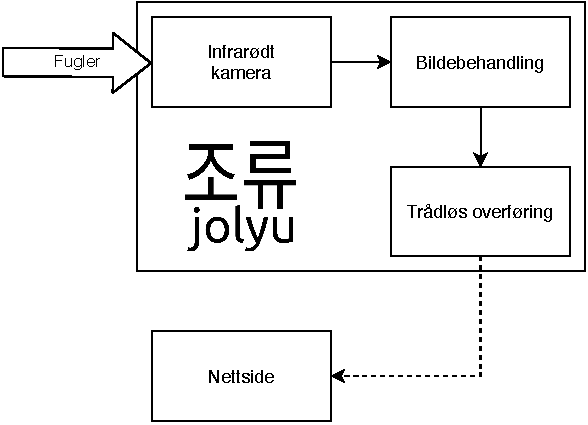
\includegraphics[width=0.75\textwidth]{konsept/Diagram_konsept.pdf}
    \caption{Blokkdiagram for konseptet.}
    \label{fig:konsept}
\end{figure}
 

$\mathbb{TEKST} \:\: \mathbb{FRA} \:\: \mathbb{INNLEVERING}$:

Systemet skal være i stand til å kunne telle fugler som flyr over et gitt område. Fuglene på himmelen skal telles og loggføres, og spores på en slik måte at en passerende fugl kun telles én gang. Dette oppnås ved at et infrarødt kamera filmer himmelen og eventuelle fuglers varmesignatur mot himmelen. Bildene analyseres i en prosesseringsenhet, som oppdager og sporer fuglene. I tillegg skal systemet inneholde sensorer for å måle værdata. Dette inkluderer nedbør, luftfuktighet, temperatur, trykk, lys, og vind. Data overføres så trådløst til en nettside, hvor den fremstilles til brukere og kan analyseres videre. Systemet kan utvides med flere kameraer for økt dekning, eller flere separate enheter. Et økt dekningsområde gir større muligheter for avansert sporing eller overvåkning av fugleaktivitet, eller for å kunne observere forskjeller i aktivitet i sanntid.




\subsection{Kamera}

Vi skal bruke et infrarødt kamera (IR-kamera) til å detektere den infrarøde strålingen fra fugler. Infrarød stråling er elektromagnetisk stråling med en bølgelengde lenger en synlig lys. (700nm-1mm). Infrarød stråling detekterer alle objekter med en temperatur over det absolutte nullpunkt (0K) og opp til 3864K. Vi er mest interessert i temperaturer rundt kroppstemperaturen til fugler (40 K https://www.sciencedirect.com/science/article/pii/030096299190122S) sett i forhold til omgivelsene fra -15 til 30 C sett i forhold til maks og minimumstemperaturer i trondheim det siste året. Dette tilsvarer bølgelenden i langbølge IR på $8-15\mu m$. Et IR-kamera bruker Stephen-Boltzmanns lov for å regne ut temperaturen til objektet $R=\epsilon \sigma T^2$ der R er infrarød stråling (W/$m^2$), T er temperatur i kelvin, $\sigma$ er boltzmanns konstant og $\epsilon$ er den termiske emissiviteten til objektet som skal måles. For fugler er denne emissiviteten målt til å være ca 0.95 (Temperature Biology
of Animals, cossin bowler 1987). 


Vi bruker et infrarødt kamera som ser etter varmesignaturen til fugler. hovedsensor for detektering av fugler. Kameraet skal gi prosseseringsenheten en kontinuerlig sendig av video.


\subsection{Deteksjon}
Systemet skal kunne detektere fugler fra en kontinuerlig videostrømm. Fuglene skal 



\subsection{Nettside}




\section{Design}
\label{sec:design}
\textit{Her kommer detaljene om \textbf{hvordan} en har tenkt at konseptet skal kunne fungere. Det er fremdeles snakk om prinsipper og ideer, ikke fysisk realisering og komponentvalg.}

Systemet har en sentral prosesseringsenhet som styrer alle undersystemene som kamera, værstasjon og eksterntilkobling. 

Systemet skal ha en sentral prosesseringsenhet som styrer to undersystemer; kamera og værstasjonen. I tillegg skal denne ha eksterntilkobling til databasen og nettsiden, sammen med lokal lagring for backup. 

Deteksjon
Prosesseringsenheten vil mota en kontinuerlig strøm av video fra kameraet. Her vil vert bilde bli behandlet internt for fugler. I tillegg skal bildene ses på kontinuerlig. Dvs om vi detekterer en fugl på bilde n og på bilde n+1 så er det en stor sannsynlighet for at dette er samme fugl. Da skal systemet forholde seg til dette og finne banen fuglen tar. 



\subsection{Blob-detection}




\subsection{}

\section{Implementering}
\label{sec:implementering}



%Overordnet består systemet av to delsystemer. Det ene delsystemet detekterer og sporer fugleaktivitet med et varmekamera, og det andre delsystemet henter inn værdata. Begge disse systemene sender data til en prosesseringsenhet, som så prosesserer dataen og sender det videre til en database, før det blir framstilt på en nettside. \todo{ganske gjentagende fra kap 3, mulig sløyfe}


\subsection{Prosesseringsenhet}\label{sec:impl:prosessor}

Til databehandling brukes en Raspberry Pi (heretter kalt Pi-en). 
Dette er en liten datamaskin på ett enkelt kretskort, men som tilbyr nok minne og prosesseringskraft til systemets formål. 
Dette tilfredsstiller systemkrav \idref{id:prosessor}. 
Pi-en utfører all bildebehandling samt prosessering av værdata og bruker trådløse kommunikasjonsegenskaper til overføring av data til databasen. 
Pi-en er modell 4B, med 4GB RAM og en 64-bits prosessor \cite{raspberry}. 
Operativsystemet som brukes er Raspbian Buster med desktop \cite{raspbian}, som er optimalisert for bruk på Pi-en.

\begin{figure}[H]
    \centering
    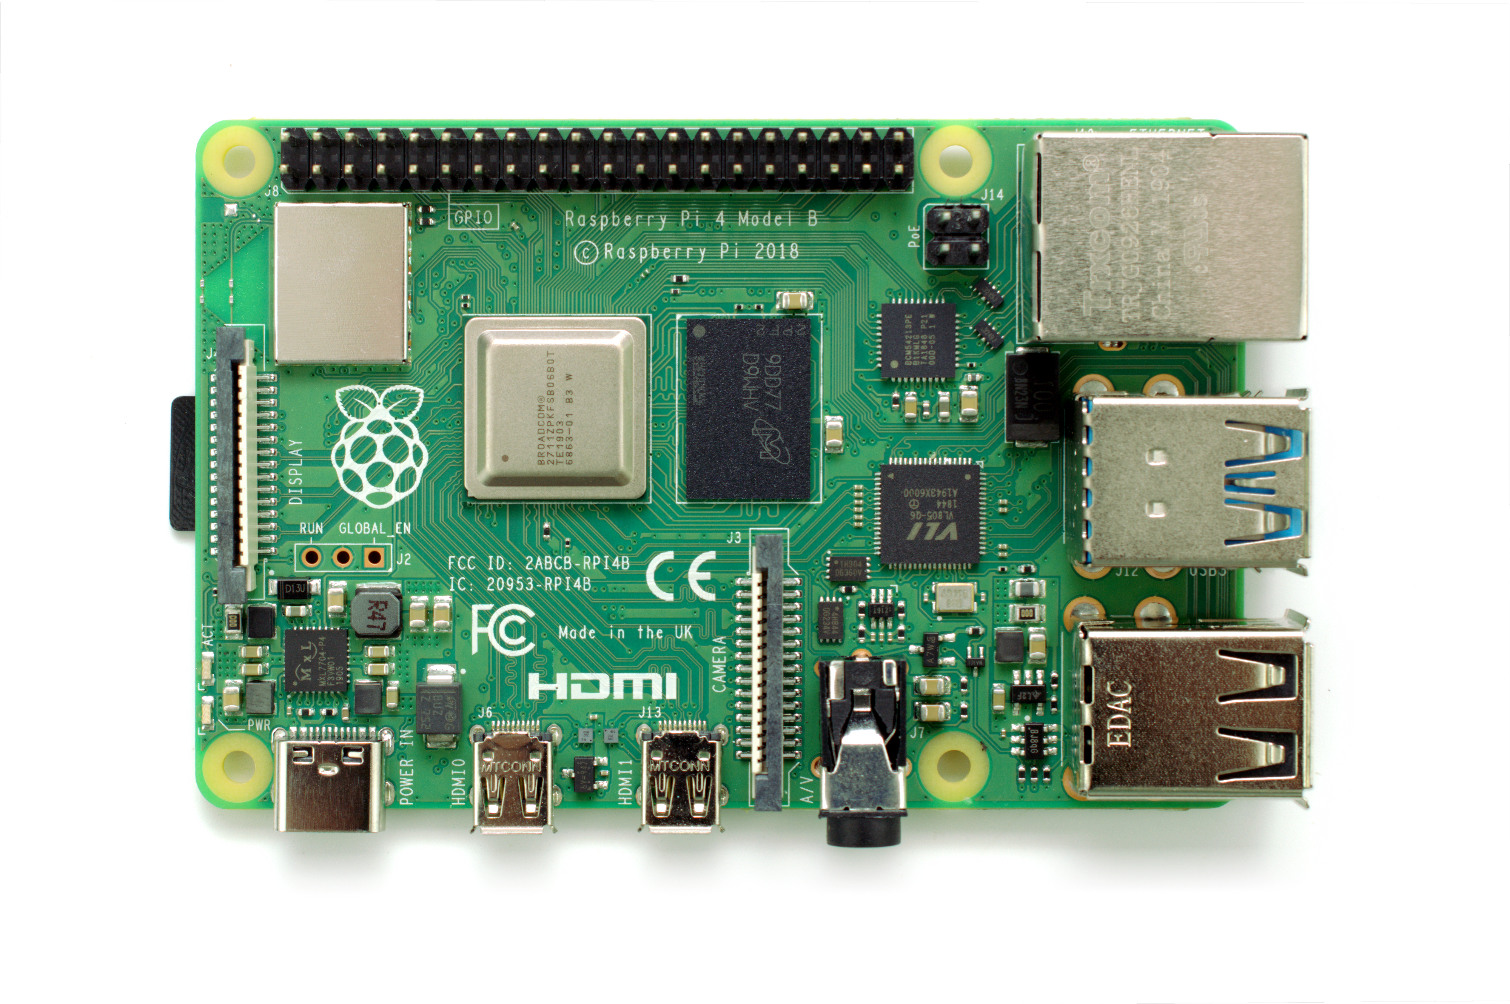
\includegraphics[width=0.6\textwidth]{implementering/pi4.png}
    \caption{Prosesseringsenheten, en Raspberry Pi 4B.}
    \label{fig:pi}
\end{figure}

%en referanse til Pi4? datablad elns?

\subsection{IR-kamera}\label{sec:impl:kamera}

Det infrarøde kameraet som benyttes er et FLIR C3-kamera.
Kameraet er håndholdt, men kan også koblet til en datamaskin, her Pi-en. 
Kameraet har en IR-sensor med synsvinkel på $41\degree\ \times\ 31\degree$, bilderate på 9 Hz, og kan detektere temperaturforskjeller på under $\SI{0.1}{\celsius}$. 
Kameraet vil kontinuerlig ta bilder med en valgbar frekvens, som optimaliseres for å gi best mulig deteksjon. 
Samtidig kan denne begrenses slik at bildebehandlingen ikke blir overbelastet. 
Bildene overføres til Pi-en via en USB-kabel som definert i systemkrav \idref{id:internoverføring}.


\begin{figure}[H]
    \centering
    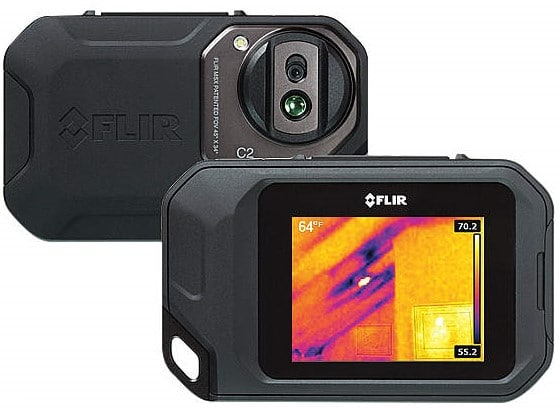
\includegraphics[width=0.5\textwidth]{implementering/c3.png}
    \caption{IR-kameraet som systemet bruker, en FLIR C3.}
    \label{fig:c3}
\end{figure}


\subsection{Programvare}\label{sec:impl:programvare} 

Hovedprogrammet kjører på Pi-en og har som mål å analysere bildestrømmen fra kamera og sende informasjon om antall fugler til en database.
Til bildebehandlingen brukes Python-rammeverket \textit{OpenCV} \cite{OpenCV}. 
\textit{OpenCV} er laget for å gi utviklere rask og enkel tilgang til avanserte algoritmer innen maskinlæring og datasyn.
Dette rammeverket kan dermed brukes til bilderprosessering i form av filtrering, deteksjon av objekter og sporing, kalt \textit{tracking}, i sanntid.

Den overordnede flyten til programmet er vist i \autoref{fig:hovedprogram}. 
Først kjører programmet gjennom en oppstartsprosedyre før det går inn i en løkke med sykliske hendelser.

\begin{figure}[H]
    \centering
    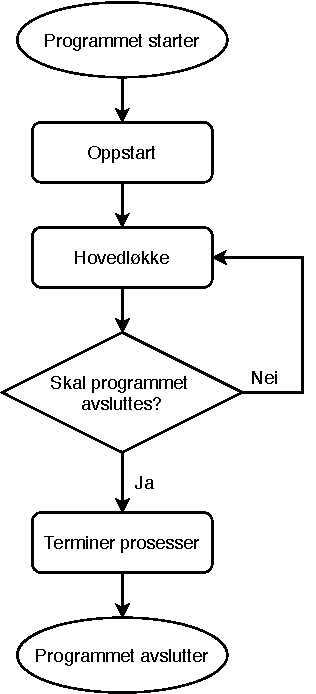
\includegraphics[width=0.2\textwidth]{implementering/Program/hovedprogram.pdf}
    \caption{Flytskjema for programmet.}
    \label{fig:hovedprogram}
\end{figure}
I oppstartsfasen initialiseres en loggfil og en link til kameraet, som vist i flytskjema i \autoref{fig:hovedprogram_oppstart}. Loggfilen er beskrevet i beskrevet i \autoref{sec:impl:programvare:logging}.

\begin{figure}[H]
    \centering
    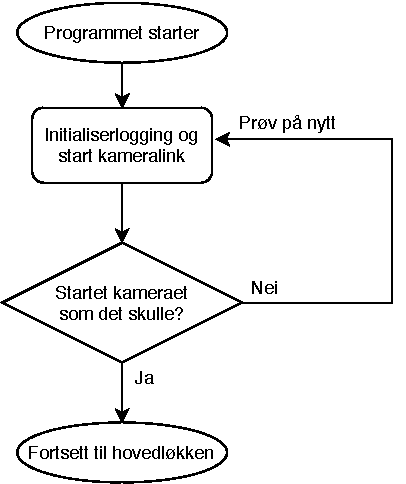
\includegraphics[width=0.3\textwidth]{implementering/Program/oppstart.pdf}
    \caption{Flytskjema for oppsettet til programmet.}
    \label{fig:hovedprogram_oppstart}
\end{figure}

Programmet fortsetter så å kjøre gjennom en rekke sykliske hendelser for bildegjenkjenning og tracking. 
Dette krever at man tar i bruk flere av de avanserte algoritmene \textit{OpenCV} tilbyr.
Ytterligere informasjon om bildeprosessering i \autoref{sec:impl:programvare:bildepro}. 
Flyten til hovedløkken kan sees i \autoref{fig:hovedprogram_loop}.

\begin{figure}[H]
    \centering
    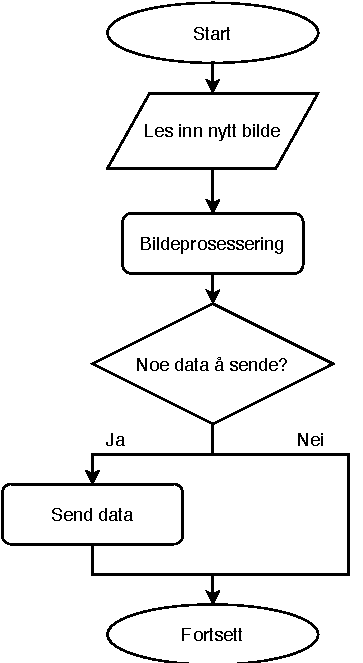
\includegraphics[width=0.3\textwidth]{implementering/Program/main_loop.pdf}
    \caption{Flytskjema til hovedløkken.}
    \label{fig:hovedprogram_loop}
\end{figure}

\textit{OpenCV} har en innbygd funksjon for å lese inn videostrømmer, slik at IR-kameraet kan benyttes som om det var et vanlig webkamera. 
Det er altså forholdsvis enkelt å lese en bildestrøm fra kameraet med Pi-en, og kode for dette er vist i \autoref{code:impl:programvare:bildestrøm}. 
Problemet blir dermed i hovedsak å prosessere og analysere disse bildene for å kunne gjenkjenne \textit{blobs} og spore disse mellom bildene.

\begin{listing}[!htb]
\begin{minted}{python}
    vc = cv2.VideoCapture(0)            #starter bildestrøm fra kamera
    
    if vc.isOpened():                   #sjekker om kameraet er åpnet
        rval, frame = vc.read()         #leser bilde fra kamera
    else:
        rval = False                    #setter rval til False fordi kameraet ikke ble åpnet
    
\end{minted}
\caption{Kodeeksempelet viser hvordan man kan bruke \textit{OpenCV} for å hente inn bilder fra en videostrøm.}
\label{code:impl:programvare:bildestrøm}
\end{listing}


\subsubsection{Bildeprosessering}\label{sec:impl:programvare:bildepro}

Det å få en datamaskin til å kjenne igjen et spesifikt objekt i et bilde, er en kompisert problemstilling ingeniører har jobbet med i mange år.
\textit{OpenCV} tilbyr en god del verktøy som muliggjør nettopp dette.

Flyten for bildeprosesseringen er illustrert i \autoref{fig:bildeprosessering}.

\begin{figure}[H]
    \centering
    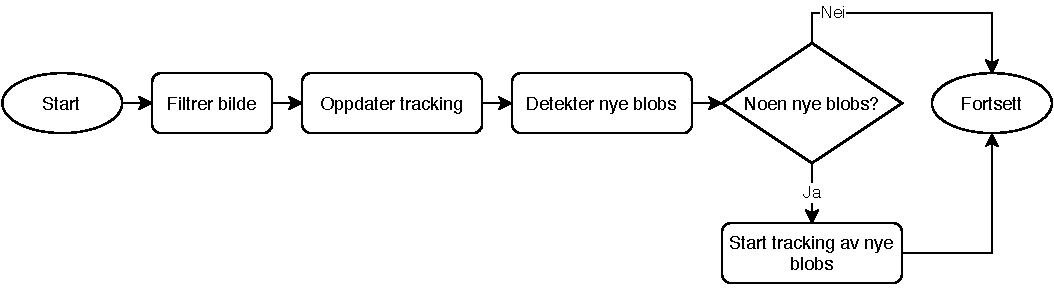
\includegraphics[width=0.3\textwidth]{implementering/Program/bildepros.pdf}
    \caption{Flyten til bildeprosesseringen.}
    \label{fig:bildeprosessering}
\end{figure}

For å lettere og mer presist kunne analysere \textit{blobs} må bildene filtreres. 
Dette er beskrevet i \autoref{sec:impl:programvare:filtrering}. 
Deretter kan man utføre \textit{blob-deteksjon} (se \autoref{sec:impl:programvare:blob-detection}) og \textit{tracking} (se \autoref{sec:impl:programvare:tracking}). 
Dette gjøres ved at man først kjører trackinalgoritmen for å spore blobs fra tidligere bilder, før man kjører blob-deteksjon og starter tracking av nye blobs. 

\subsubsection{Filtrering}\label{sec:impl:programvare:filtrering}
For å oppnå best mulig deteksjon av fugler, filtreres bildene for å redusere støy og annen unyttig informasjon. 
Ideelt sett vil fulgen og bakgrunnen på bildet ha helt forskjellige farger med tydelig konstrast, da det gjør det lettest å detektere fuglene. 
Filtreringsalgoritmen prøver å oppnå dette idealet. 

Algoritmen som gjør hoveddelen av filteringen, heter Otsus metode\cite{otsu}. 
Algoritmen regner ut en terskelverdi for hvert bilde, som så kan brukes for å konvertere bildet om fra gråskala til sort-hvitt. 
Bilde blir gjort om til gråskala ved å bruke funksjonen \python{cvtColor()}, som er en innebygd funksjon i \textit{OpenCV}. Den gjør bilde om til gråskala ved ta et vektet gjennomsnitt av fargeverdiene \cite{cvtColor}.


Otsus metode fungerer ved å først dele bildet inne i to klasser, bakgrunn og forgrunn. 
Deretter utregnes variansen i fargeverdier i begge klassene og mellom klassene. 
En terskelverdi velges så slik at variansen innad i klassen minimeres, og variansen mellom klassene maksimere. 


Den matematiske sammenhengen i \eqref{Binarization}, sier hvordan terskelverdien brukes til å forvandle bilde om til sort-hvit. 
I den sammenhengen er $1$ svart og $0$ hvit. 
Funksjonen $f(x,y)$ gir fargeverdien til pikslene i gråskalabilde og funksjonen $dst(x,y)$ gir fargeverdiene til bilde i sort-hvit. 
Variabelen $T$ er terskelverdien. 
For mer utdypning på hvordan algoritmen fungerer se \cite{otsu}.
Implementasjonen av algoritmen er gitt i \autoref{code:impl:programvare:manual_otsu_binary}

\begin{align}
    dst(x,y)= \begin{cases} 
        1 \text{ hvis } f(x,y) > T\\
        0 \text{ ellers.}
   \end{cases}\label{Binarization}
\end{align}


\begin{listing}[!htb]
\begin{minted}{python}
def manual_otsu_binary(img):
    '''Otsu binarization function by calculating threshold'''
    #gaussisk uskarphet (eng: gaussian blur)
    blur = cv2.GaussianBlur(img, (KERNEL_SIZE, KERNEL_SIZE), 0)  
    
    #finner den normaliserte_histogrammet for den kumulativedistribusjonsfunksjonen.
    hist = cv2.calcHist([blur], [0], None, [256], [0, 256])
    hist_norm = hist.ravel() / hist.max()
    Q = hist_norm.cumsum()
    bins = np.arange(256)
    fn_min = np.inf
    thresh = -1

    for i in range(1, 255):
        p1, p2 = np.hsplit(hist_norm, [i])  #sannsynligheter 
        q1 = Q[i]
        q2 = Q[255] - q1  # kumulative sum av klassene
        b1, b2 = np.hsplit(bins, [i])  # vekter 
        
        # finner middelverdiene og variansene
        m1 = np.sum(p1 * b1) / q1
        m2 = np.sum(p2 * b2) / q2
        v1, v2 = np.sum(((b1 - m1) ** 2) * p1) / q1, np.sum(((b2 - m2) ** 2) * p2) / q2
        # Renger ut minimum for funksjonen. 
        fn = v1 * q1 + v2 * q2
        if fn < fn_min:
            fn_min = fn
            thresh = i

    _, img_thresh1 = cv2.threshold(img, thresh, 255, cv2.THRESH_BINARY)
    return img_thresh1
    
\end{minted}
\caption{Implementering av Otsus metode. }
\label{code:impl:programvare:manual_otsu_binary}
\end{listing}
\todo{vi må dobbeltsjekke matten til det filteret det, for det er mulig det ikke stemmer 100 \%}

Etter Otzus metode kan man så utføre \textit{morphology}-transformasjoner. 
Dette er funksjoner som er implementert i \textit{OpenCV}-rammeverket. 
Her ønsker man å utføre \textit{erosion} og \textit{dialation}.
\textit{Erosion} brukes for å filtrere bort støy (white noise), men samtidig krymper det objektet innover fra kantetne. Dette problemet løser \textit{OpenCV} ved \textit{dialation}, som igjen øker størrelsen til objektet.
\textit{OpenCV} har implementerte funksjoner som bruker kombinasjoner av disse til å filtrere bort støy. 
\textit{Opening} brukes for å fjerne støy fra en bakgrunn, mens \textit{closing} brukes i det motsatte tilfellet for å fjerne små hull i et objekt (\textit{blobs}) i forgrunnen. Disse kjøres etter otzu-filteret for å filtrere bort eventuell støy fra de resulterende bildene.

%opencv dokumentasjon om morphology https://docs.opencv.org/trunk/d9/d61/tutorial_py_morphological_ops.html

\subsubsection{Blob-deteksjon}\label{sec:impl:programvare:blob-detection}

Rammeverket \textit{OpenCV} brukes også til blob-deteksjon. 
Funksjonen som brukes fra \textit{OpenCV} til dette, er \python{SimpleBlobDetector()}. 
Den returnerer et objekt av \python{detector}-klassen. 
Klassen inneholder alle parametere til blob-deteksjonen, det vil si hvilke krav vi stiller til hva som regnes som en blob. 
I tillegg inneholder klassen en medlemsfunksjon, \python{detect}, som finner alle blobene i bildet og returnerer en liste med koordinatene til disse. 
Kodeeksempel \ref{code:impl:programvare:blob_detection_func} viser hvordan disse funksjonene er brukt. Implementasjonen av funksjonene og klassen finnes i Githuben til \textit{OpenCV} \cite{OpencCV_Git}.
\begin{listing}[!htb]
\begin{minted}{python}
#blob-deteksjon parametere:
MAX_AREA = 5000
MIN_AREA = 10

def init_blob_detector():
    '''Setup SimpleBlobDetector parameters'''
    params = cv2.SimpleBlobDetector_Params()

    # Forandrer tersklene for areal
    params.maxArea = MAX_AREA
    params.minArea = MIN_AREA

    detector = cv2.SimpleBlobDetector_create(params)    #create detector

    return detector
    
def blob_detection(img):
    '''Function to detect blobs. Returns list of keypoints'''

    detector = init_blob_detector() |\label{code:impl:programvare:blob_detection_func:line:init_blob}|    #oppretter detektor med parametere for blobs
    keyPoints = detector.detect(img)    #analyserer og lager en liste med nøkkelpunkter
    
    return keyPoints
    
\end{minted}
\caption{Implementasjon av blob-deteksjon. Merk at koden her er noe redigert for å være mer lesevennlig. Blant annet brukes flere ulike parametere. }
\label{code:impl:programvare:blob_detection_func}
\end{listing}

Som vi kan se i \autoref{code:impl:programvare:blob_detection_func}, oppretter \python{init_blob_detector()}-funksjonen i linje \ref{code:impl:programvare:blob_detection_func:line:init_blob} en \python{detektor}, hvor vi fritt kan endre på en rekke parametere, som for eksempel areal. 
Til slutt returnerer den en \python{detector} med parameterne satt til det vi ønsket at de skal være. 
Funksjonen \python{blob_detection()} oppretter en slik \python{detektor}ved å kalle på \python{init_blob_detector()}, og bruker den innebygde \python{detect}-funksjonen til \textit{OpenCV} til å analysere bildet. 

Den returnerer så en liste over \textit{nøkkelpunkter}(''keypoints''). 
Et \textit{nøkkelpunkt} er objekt som inneholder koordinatene til en blob samt radiusen. 
Videre brukes \python{blob_detection()} hver gang vi skal finne \textit{nøkkelpunktene} i et bilde.

\subsubsection{Tracking}\label{sec:impl:programvare:tracking}
For å unngå at programmet teller samme fugl flere ganger, brukes \textit{tracking}. 
Måten trackingen fungerer er at en tracker konstrueres og gis koordinater til et område på skjermen der det finnes et objekt. 
Dette objektet vil \textit{trackingen} kjenne igjen når neste bilde kommer, og den vil klare å følge objektet gjennom videostrømmen.
Siden det kan være flere fugler i bildet samtidig, må det være mulig å \textit{tracke} alle uavhengig av hverandre. 
Dette gjøres ved å lage et \textit{multi-tracker} objekt som samler flere \textit{trackere}. 
Hver av disse \textit{trackerene} følger forskjellige fugler.
Ved bruk av flere \textit{trackere}, er det viktig at hver fugl kun \textit{trackes} en gang. 
Dette er for å unngå at den samme fuglen telles flere ganger. 
Dersom et objekt allerede har en \textit{tracker}, vil \textit{multi-trackeren} passe på at det ikke oprettes en ny \textit{tracker} for samme objekt.
% Gammel setning: Ved å ikke opprette en tracker der det allerede finnes en, vil det unngås.

Når en fugl skal trackes er koordinatene til fuglen i bildet nødvendig. 
Dette hentes fra blob-detection koden. 
Blob-detection-koden returnerer en liste med \textit{nøkkelpunkter}. 
Disse inneholder senter og radius til blobbene som er i bildet.
\textit{Trackerfunksjonen}, som skal \textit{tracke} \textit{blobbene}, tar derimot inn en firkantet boks som må omslutte blobben helt.
For at trackingen skal fungere optimalt må boksen være en del større enn \textit{blobben}.
Derfor er det behov for en funksjon som kan gjøre om \textit{nøkkelpunkter} til bokser. 
Dette er vist i \autoref{code:keypointsToBoxes}. 
Funksjonen \python{KeypointsToBoxes(keypoint)} returnerer en liste som inneholder all info om boksene som trengs til \textit{trackingen}.

\begin{listing}[!htb]
\begin{minted}{python}
    def KeypointsToBoxes(keypoints):
        boxes = []  #liste for bokser rundt alle keypoints 
        for keypoint in keypoints:
        #boksene lages ved hjelp av sentrum og størrelsen på blobbene
            point = keypoint.pt
            size = 10 + 3*int(keypoint.size)
            box = (int(point[0])- (size/2),int(point[1]) - (size/2), size, size)
            boxes.append(box)
        return boxes
\end{minted}
\caption{Kode som viser hvordan keypoints fra blob-detection blir gjort om til bokser som kan brukes til trackingen.}
\label{code:keypointsToBoxes}
\end{listing}

Når alle \textit{nøkkelpunkter} er gjort om til bokser, må det identifiseres hvilke \textit{blobs} som allerede \textit{trackes}. 
Det kan gjøres ved å sjekke om midten av noen av \textit{blobbene} ligger innenfor boksen til en blob som allerede \textit{trackes}. 
Hvis den gjør det må ikke \textit{blobben} \textit{trackes} på nytt. 
Funksjon\newline \python{removeTrackedBlobs(keypoints, boxes)} i \autoref{code:removeTrackedBlobs} viser hvordan dette gjøres.
I denne funksjonen blir nøkkelpunktene til \textit{blobbene} som allerede \textit{trackes} fjernet fra listen. 
\textit{Nøkkelpunktene} til de resterende \textit{blobbene} blir returnert.

\begin{listing}[!htb]
\begin{minted}{python}
    def removeTrackedBlobs(keypoints, boxes):
        #newKeypoints: liste med nye blobs, diff: for allerede tracka blobs
        newKeypoints = []
        diff = []
        try:
        #Sjekker om blobs er nye. Legges til i tilhørende liste
            for points in keypoints:
                x = points.pt[0]
                y = points.pt[1]
                for box in boxes:
                    xb,yb,wb,hb = box
                    if xb<x and x<xb+wb and yb<y and y<yb+hb:
                        diff.append(points)
            for point in keypoints:
                if point not in diff:
                    newKeypoints.append(point)
        except:
            pass
        #returnerer alle nye blobs
        return newKeypoints
\end{minted}
\caption{Kodeeksempelet viser hvordan det sjekkes om blobs er nye eller om de trackes fra et tidligere bilde.}
\label{code:removeTrackedBlobs}
\end{listing}

\textit{OpenCV} har flere funksjoner som hjelper til med denne \textit{trackingen}, og har flere forskjellige metoder for \textit{tracking} som varierer i nøyaktighet og tidsbruk.
For å opprette en \textit{tracker} av en av disse \textit{trackertypene} kalles funksjonen \python{createTrackerByName(trackerType)}, der \python{trackerType} er hvilken type \textit{tracker} som blir brukt. En rask og god \textit{tracker} som er valgt i dette prosjektet er ''CSRT-trackeren''. 
Etter trackeren er konstruert, må den initialiseres.
Dette gjøres ved å si hvilket bilde blobben er i og koordinater til en boks som skal omslutte blobben. 
Siden det kan være flere fugler i et bilde, er det nødvendig å kunne lage flere trackere, og lagre disse sammen.

\textit{OpenCV} har en \textit{multitrackerklasse}, men denne er ikke optimal, da det ikke kan slettes \textit{trackere} fra et \textit{multitracker-objekt}. 
Derfor er en ny klasse implementert med de ønskede egenskapene. 
Denne klassen er kalt \python{NewTracker} og en del av implementeringen av denne klassen kan sees i \autoref{code:newTracker}. 
Klassen består av to lister og en rekke medlemsfunksjoner. 
Listen \python{trackers} består av enkle \textit{trackere}, og listen \python{trackerFail} består av heltall som forteller i hvor mange bilder etter hverandre \textit{trackeren} har mislyktes med å følge en \textit{blob}. 
Når \textit{blobdeteksjons} algoritmen har kjørt, legges det til trackere til alle nye \textit{blobs} med medlemsfunksjonen \python{add}.
I tillegg har \python{NewTracker}-klassen medlemsfunksjonene \python{pop} og \python{update}\cite{GitHub}. 
Funksjonen \python{pop} fjerner \textit{trackere}, og \python{update} oppdaterer alle \textit{trackere}. 
I tillegg til å oppdatere \textit{trackerene}, vil \python{update}-funksjonen inkrementere listeelementene i \python{trackerFail} som hører til trackere som mislyktes med sporingen sin.
Dersom \textit{trackeren} klarte å følge \textit{blobben} blir tilhørende \python{trackerFail}-element satt til $0$. 
Alle \textit{trackere} som ikke har detektert blobben sin i fem bilder på rad, vil fjernes fra \textit{multitrackeren}. Funksjonen \python{update} returnerer også en liste med koordinatene til alle \textit{trackere}.

\todo{hva skjer når to blobs krysser hverandre?}

\begin{listing}[!htb]
\begin{minted}{python}
    class NewTracker():                     
        def __init__(self):
        #objektet består av to lister
        #En med trackerne, og en som vet hvor lenge en tracker har vært ugyldig
            self.trackers = []             
            self.trackerFail = []
    
        def add(self, trackerObj):
        #når en ny tracker legges til, legges den inn i self.trackers
        #i tillegg får den et element i trackerFail-lista,
        #som viser at den har vært ugyldig i 0 bilder
            self.trackers.append(trackerObj)
            self.trackerFail.append(0)
\end{minted}
\caption{Konstruktøren og add-funksjonen til multitrackeren.}
\label{code:newTracker}
\end{listing}


\subsubsection{Logging}\label{sec:impl:programvare:logging}
Det er ikke alltid systemet fungerer som det skal.
Derfor er det svært nyttig å ha en loggfil der all viktig informasjon om programmets aktiviteter lagres. 
Både operasjonene programmet gjør vellykket og det programmet ikke har fått til, blir lagt til i loggfilen. 
Begge heldelser er nyttig informasjon. 
Alt som blir lagt til i logging-fila, blir også merket med hvor viktig informasjonen er, for eksempel \python{INFO} eller \python{CRITICAL}. 

\subsection{Værstasjon}\label{sec:impl:vaer}

Værstasjonen vil måle temperatur, trykk og luftfuktighet, i tillegg til vindhastighet, vindretning og nedbørsmengde. 
All dataen sendes via et egendesignet kretskort til prosesseringsenheten, som prosesserer dataen og sender det videre til databasen for så å bli gjort tilgjengelig på nettsiden.


\subsubsection{Trykk, temperatur, luftfuktighet}\label{sec:impl:vaer:ttl}

All luftdataen hentes fra en BME280-sensor fra Bosch \cite{bme280}, som måler både temperatur, trykk og fuktighet i lufta. 
Kommunikasjonen mellom sensoren og Raspberry Pi-en foregår over en I2C-protokoll, en synkron, seriell bussprotokoll \cite{i2c}. 
Denne bussprotokollen tillater toveiskommunikasjon, og bruker 7-bits adresser. 
I2C tillater dermed opp til 128 enheter ved bruk av kun to ledninger. 
Figur \ref{fig:luftsensor_krets-} under viser kretstegning av luftsensoren.

\begin{figure}[H]
    \centering
    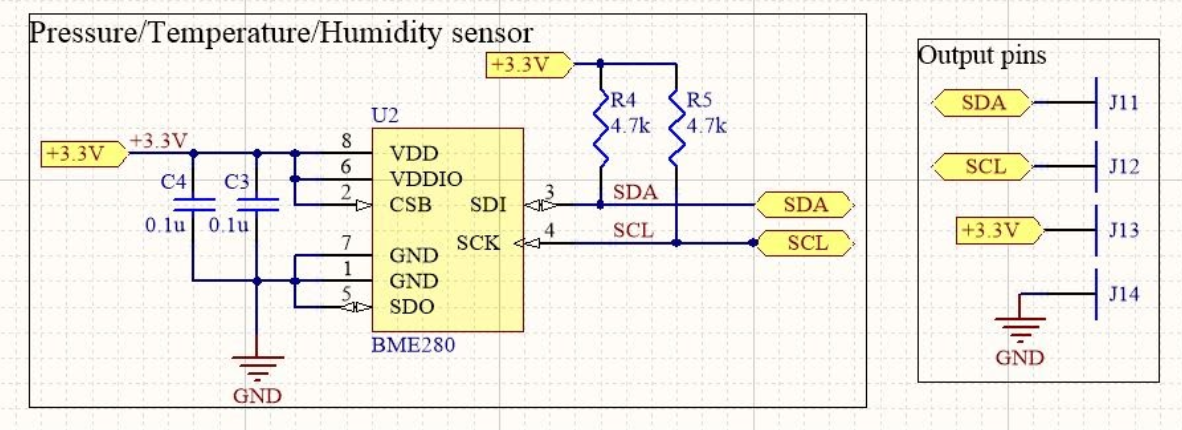
\includegraphics[width=0.9\textwidth]{implementering/luftsensor_krets.png}
    \caption{Kretsskjema for luftsensoren.}
    \label{fig:luftsensor_krets-}
\end{figure}

De eneste eksterne komponentene BME280-sensoren, $U2$, trenger rundt seg, er en kondensator ved hver av de to spenningsinngangene \texttt{VDD} og \texttt{VDDIO}, $C3$ og $C4$, og en opptrekksmotstand (eng: pull-up resistor) til databussen \texttt{SDA} og en til klokkebussen \texttt{SCL}, henholdsvis $R4$ og $R5$. Figur \ref{fig:luftsensor_3d} under viser 3d-modell av kretskortet.

\begin{figure}[H]
    \centering
    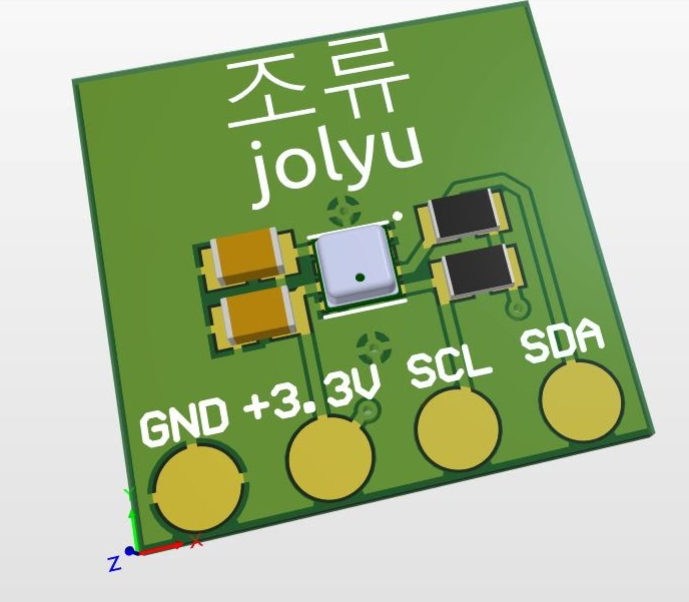
\includegraphics[width=0.5\textwidth]{implementering/luftsensor_3d.png}
    \caption{3D-modell av luftsensoren.}
    \label{fig:luftsensor_3d}
\end{figure}

For å lese data fra sensoren finnes det et eget bibliotek som heter \textit{bme280lib} \cite{bme280lib}, som gjør det enkelt å lese data fra sensoren med en sample-funksjon. 
Biblioteket \textit{smbus2} \cite{smbus2} brukes også for å opprette en I2C bussforbindelse. Programme som leser dataen, ligger i bme280.py filen under \textit{Weather-station} i GitHuben\cite{GitHub}.

\subsubsection{Anemometer}\label{sec:impl:vaer:anemometer}

Anemometeret som brukes, vist i figur \ref{fig:anemometer}, måler vindhastigheten. 
Sensoren bruker en \textit{reed-bryter}, en mekanisk bryter som lukkes av et magnetisk felt. 
For hver omdreining beveger en magnet seg forbi denne bryteren, slik at den lukkes i et kort øyeblikk. 
Ved å telle antall ganger bryteren lukkes per tidsenhet, kan rotasjonshastigheten til vindmåleren beregnes. 
Dette kan igjen brukes til å regne ut vindhastigheten. 
I følge databladet\cite{weather} vil bryteren lukkes én gang i sekundet ved en vindhastighet på $\SI{2.4}{\kilo\meter\per\hour}$, som tilsvarer $\SI{0.67}{\meter\per\second}$.


\begin{figure}[H]
    \centering
    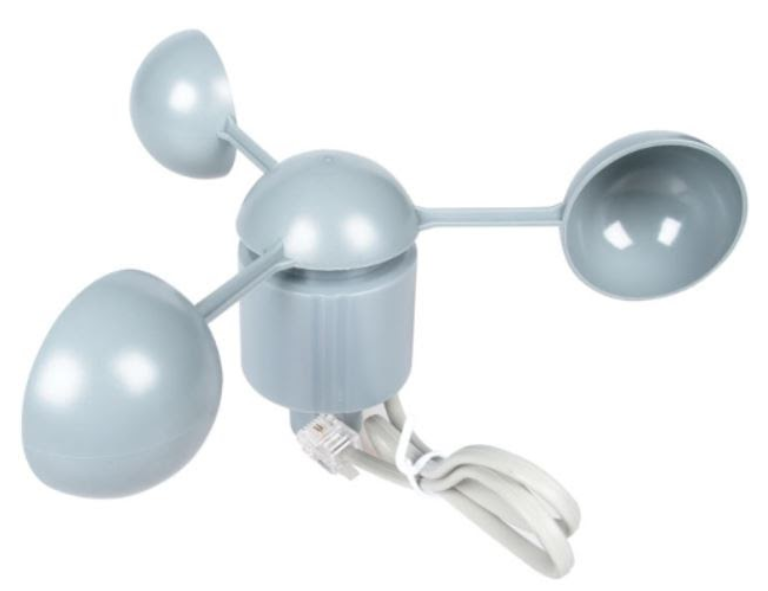
\includegraphics[width=0.5\textwidth]{implementering/anemometer.png}
    \caption{Figur av anemometeret som brukes.}
    \label{fig:anemometer}
\end{figure}

For å telle antall omdreininger, brukes klassen \python{Button} fra biblioteket \textit{gpiozero} for å registrere når reed-bryteren lukkes. Programme til anemometeret, ligger i WeatherStationMain.py under \textit{Weather-station} i GitHuben\cite{GitHub}.

%https://www.argentdata.com/files/80422_datasheet.pdf

\subsubsection{Vindretning}\label{sec:impl:vaer:vindret}

Retningsmåleren, vist i figur \ref{fig:vindretning}, består av 8 reed-brytere plassert i en sirkel slik at det er $45\degree$ mellom hver bryter \cite{weather}. 
En værhane med en påmontert magnet vil rette seg mot vinden, og vil lukke enten en bryter eller to nabobrytere om gangen, avhengig av posisjonen.
Dette resulterer i totalt 16 posisjonskombinasjoner, og dermed en nøyaktighet på $\pm 11.25\degree$. 
De 16 ulike kombinasjonene vil koble signalpinen til 16 ulike motstandsverdier, som gjør at vindretingen kan leses som et analogt signal ved hjelp av en spenningsdeler for å finne retningen. 
Pi-en ikke har en innebygd analog/digital-omformer (ADC), sendes det analoge signalet via en MCP3221A5T ADC til Pi-en.
Spenningsdelingen og analog/digital-omformeren, samt programmet som henter ut dataen fra ADC-en, er diskutert nærmere i \autoref{sec:impl:vaer:kretskort}.

Når det analoge signalet fra sensoren er lest av prosesseringsenheten, brukes et \textit{dictionary}\footnote{En type uordnet liste der man lagrer data under en nøkkel(key)\cite{dictionaries}.} for å koble de ulike verdiene til ulike vinkler.
Dette ble kalibrert ved manuelt å rotere sensoren, og lese av verdien ved ulike vinkler. 
Programmet returnerer så en retningsvinkel i grader, hvor 0\degree er definert som nord. 
Programme ligger i \textit{windDirection.py} under \textit{Weather-station} i GitHuben\cite{GitHub}.

\begin{figure}[H]
    \centering
    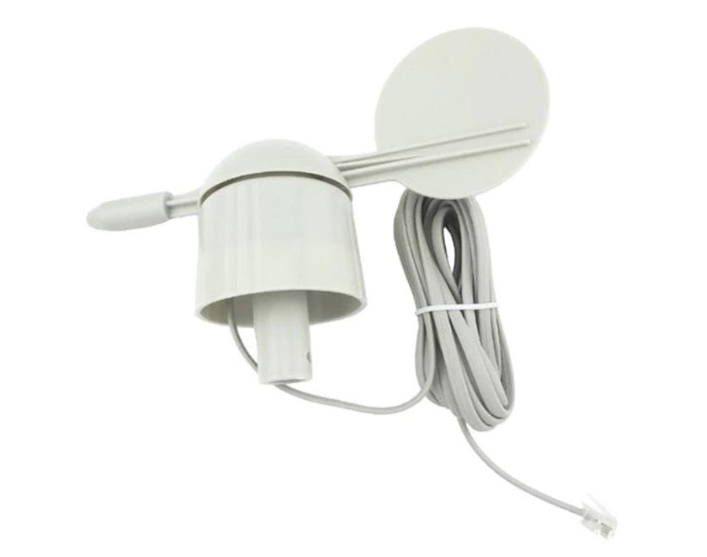
\includegraphics[width=0.5\textwidth]{implementering/vindretning.png}
    \caption{Figur av vindretningssensoren som brukes.}
    \label{fig:vindretning}
\end{figure}


\subsubsection{Nedbør}\label{sec:impl:vaer:regn}

Nedbørsmåleren består av to selvtømmende beholdere, som fylles opp og tipper over etter en gitt mengde nedbør. 
Når den ene beholderen er fylt opp og tipper over, renner vannet ut under sensoren, og den nye beholderen blir plassert under vanninntaket. 
Denne sensoren bruker også en reed-bryter, som trigges av en magnet hver gang en beholder tipper over. 
Ved å telle antall ganger bryteren lukkes og multiplisere vannmengden før en beholder tipper over, beregnes mengden nedbør som har falt i et gitt tidsrom. 
Mengden nedbør før en beholder tipper er i databladet\cite{weather} definert til å være $0,2794$mm. Figur \ref{fig:impl:vaer:regn} viser bilde av nedbørsmåleren.

\begin{figure}[H]
    \centering
    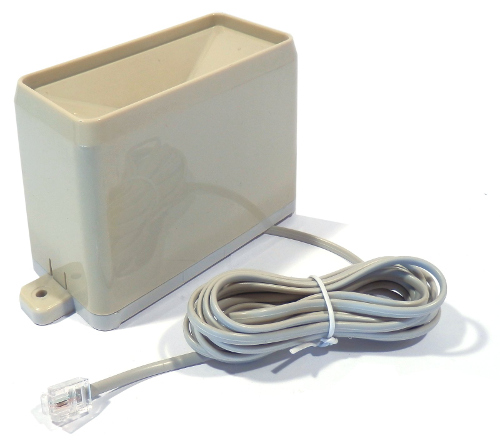
\includegraphics[width=0.5\textwidth]{implementering/rain_gauge.jpg}
    \caption{Figur av nedbørsmåleren som brukes.}
    \label{fig:impl:vaer:regn}
\end{figure}

Tilsvarende som med anemometeret i \autoref{sec:impl:vaer:anemometer}, brukes også klassen \python{Button} fra biblioteket \textit{gpiozero} her for å detektere hver gang reed-bryteren lukkes. Programme ligger i \textit{weatherStationMain.py} under \textit{Weather-station} i GitHuben\cite{GitHub}.

\subsubsection{Kretskort til sensorer}\label{sec:impl:vaer:kretskort}


For å enkelt kunne koble alle sensorene til Pi-en, brukes et egenutviklet kretskort.
Figur \ref{fig:sensorkretskort_krets} viser kretstegning til dette kretskortet.

\begin{figure}[H]
    \centering
    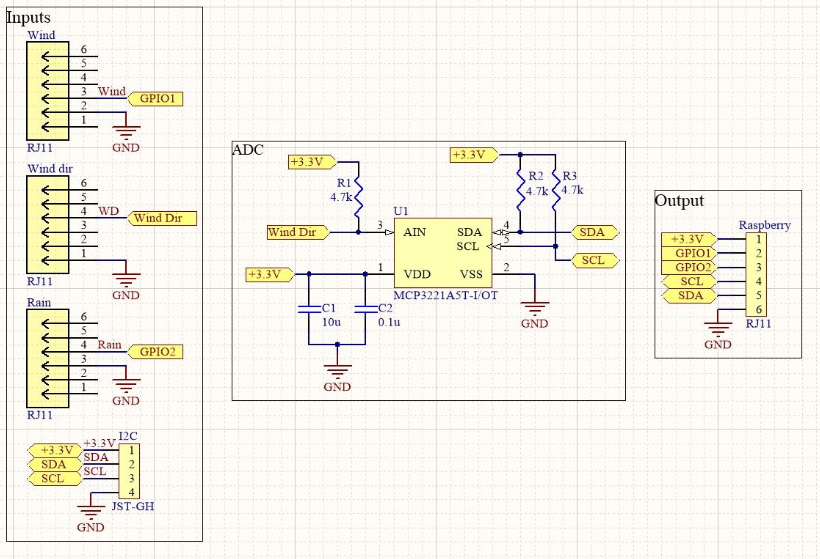
\includegraphics[width=0.8\textwidth]{implementering/sensorkretskort_krets.png}
    \caption{Kretsskjema for kretskortet til sensorene.}
    \label{fig:sensorkretskort_krets}
\end{figure}

I tillegg til kontakter for å koble til sensorene, inneholder kretskortet en motstand, $R1$, til spenningsdeleren til vindretningsensoren. 
Videre inneholder kretskortet en analog/digital-omformer, $U1$, for å digitalisere signalet fra spenningsdeleren. 
ADC-en som brukes er en MCP3221A5T fra Microchip\cite{adc}. 
Omformeren tar inn et analogt signal, og kommuniserer direkte over I2C-bussprotokollen med Pi-en. 
Opptrekksmotstander, $R2$ og $R3$, brukes også her for å trekke $SDA$ og $SCL$ bussene høye, og to kondensatorer, $C1$ og $C2$, brukes for å filtrere bort ulike støyfrekvenser fra spenningsforsyningen. Figur \ref{fig:sensorkretskort_3d} viser en 3d-modell av kretskortet.

\begin{figure}[H]
    \centering
    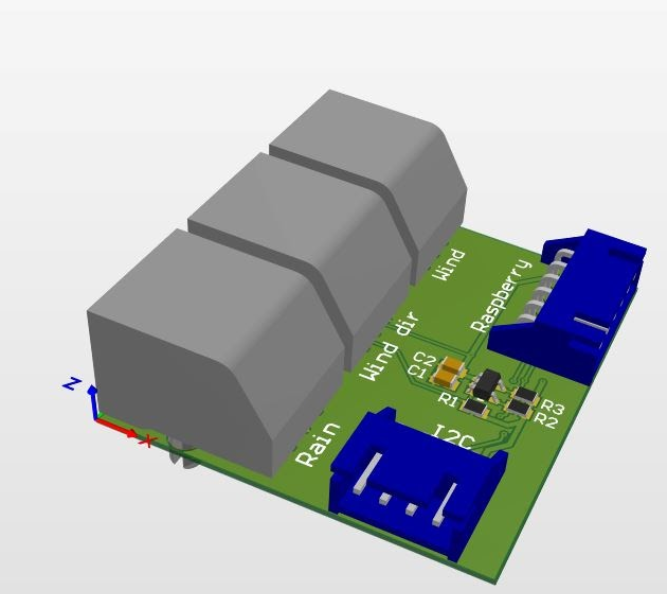
\includegraphics[width=0.5\textwidth]{implementering/sensorkretskort_3d.png}
    \caption{3d-modell av kretskortet til sensorene.}
    \label{fig:sensorkretskort_3d}
\end{figure}

For å lese data fra MCP3221A5T ADC-en, brukes igjen biblioteket \textit{smbus2}\cite{smbus2}. 
Funksjonen \\ \python{read_byte_data(address, byte)} fra dette biblioteket, brukes for enkelt å lese data fra ADC-en over I2C-protokollen. 


Luftsensoren og ADC-en til vindretningssensoren kommuniserer med prosesseringsenheten direkte via samme I2C-buss. 
GPIO pin 2 og 3 brukes til henholdsvis databussen \texttt{SDA} og klokkebuss \texttt{SCL} til kommunikasjon over I2C-bussprotokollen.
Anemometeret og nedbørssensoren kobles til henholdsvis GPIO pin 5 og 6 på Pi-en via kretskortet, som vist i \autoref{fig:kretsskjema_pi}. 

Anemometeret og nedbørsmåleren er koblet til henholdsvis GPIO pin 5 og 6 på Raspberry Pi-en, mens GPIO pin 2 og 3  3.3 volt spenning hentes også fra Raspberry Pi-en.

\begin{figure}[H]
    \centering
    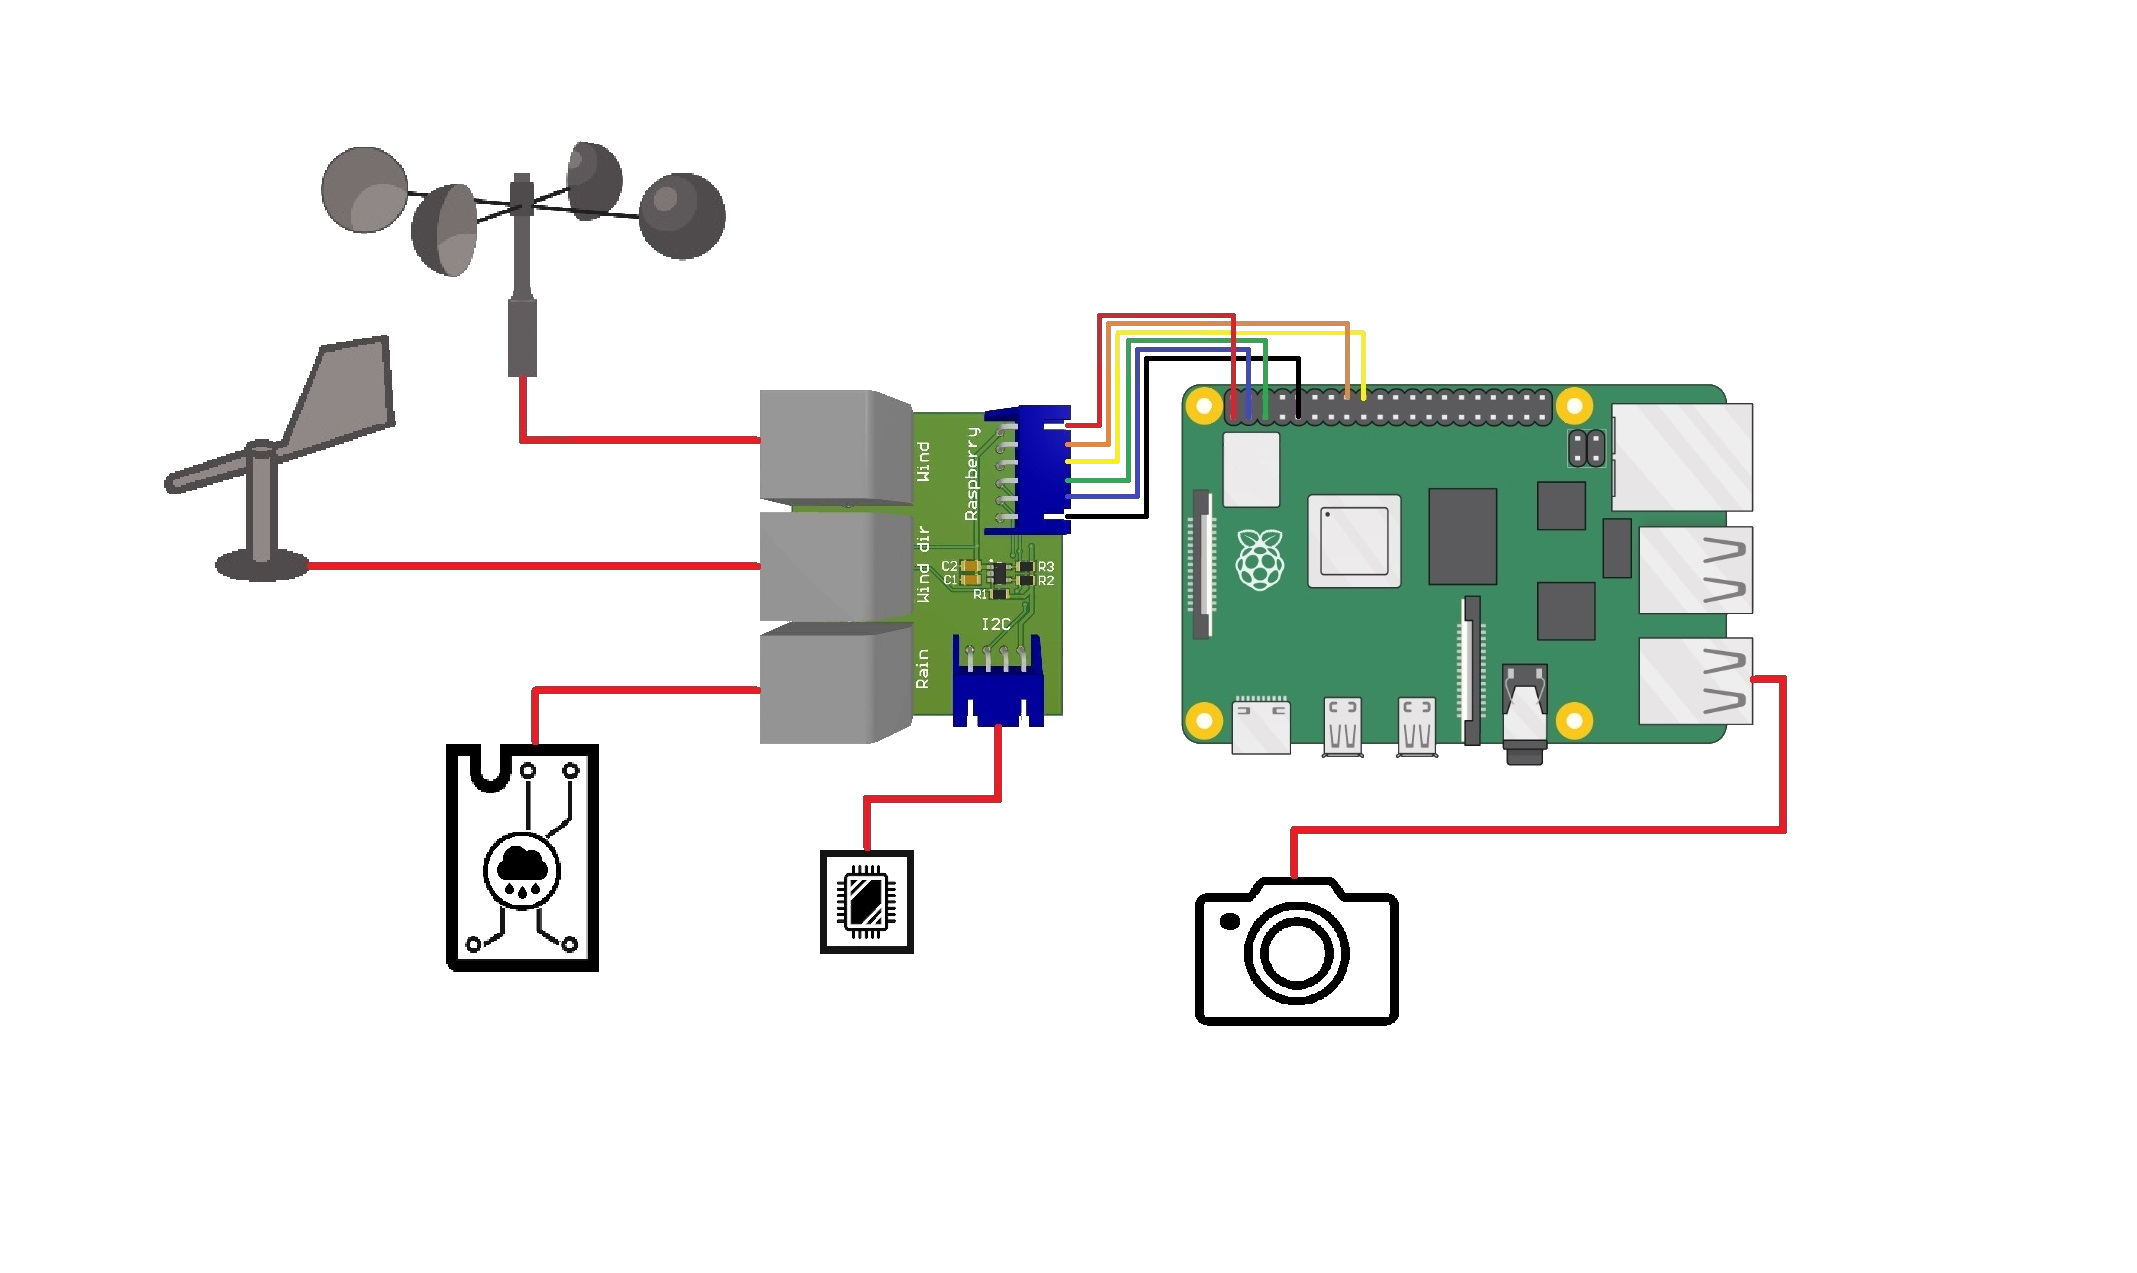
\includegraphics[width=\textwidth]{implementering/kretsskjema_pi.png}
    \caption{Figuren viser oppkoblingen av værstasjonen til prosesseringsenheten.}
    \label{fig:kretsskjema_pi}
\end{figure}
\todo{Trenger det å være så mye tekst i bildeteksten?}


\subsection{Nettside og database}\label{sec:impl:nettside}

Nettsiden har som mål å vise informasjonen som hentes inn av både fugletelleren og værstasjonen. 
Til dette brukes Python-rammeverket \textit{Dash} \cite{dash}. 
Dash er laget spesifikt for å vise og prosessere store mengder data i enkle grafer og oppgi disse på en statisk nettside. 
Se \autoref{fig:nettside:nettside}  for en eksempelnettside.

\begin{figure}[!htbp]
    \centering
    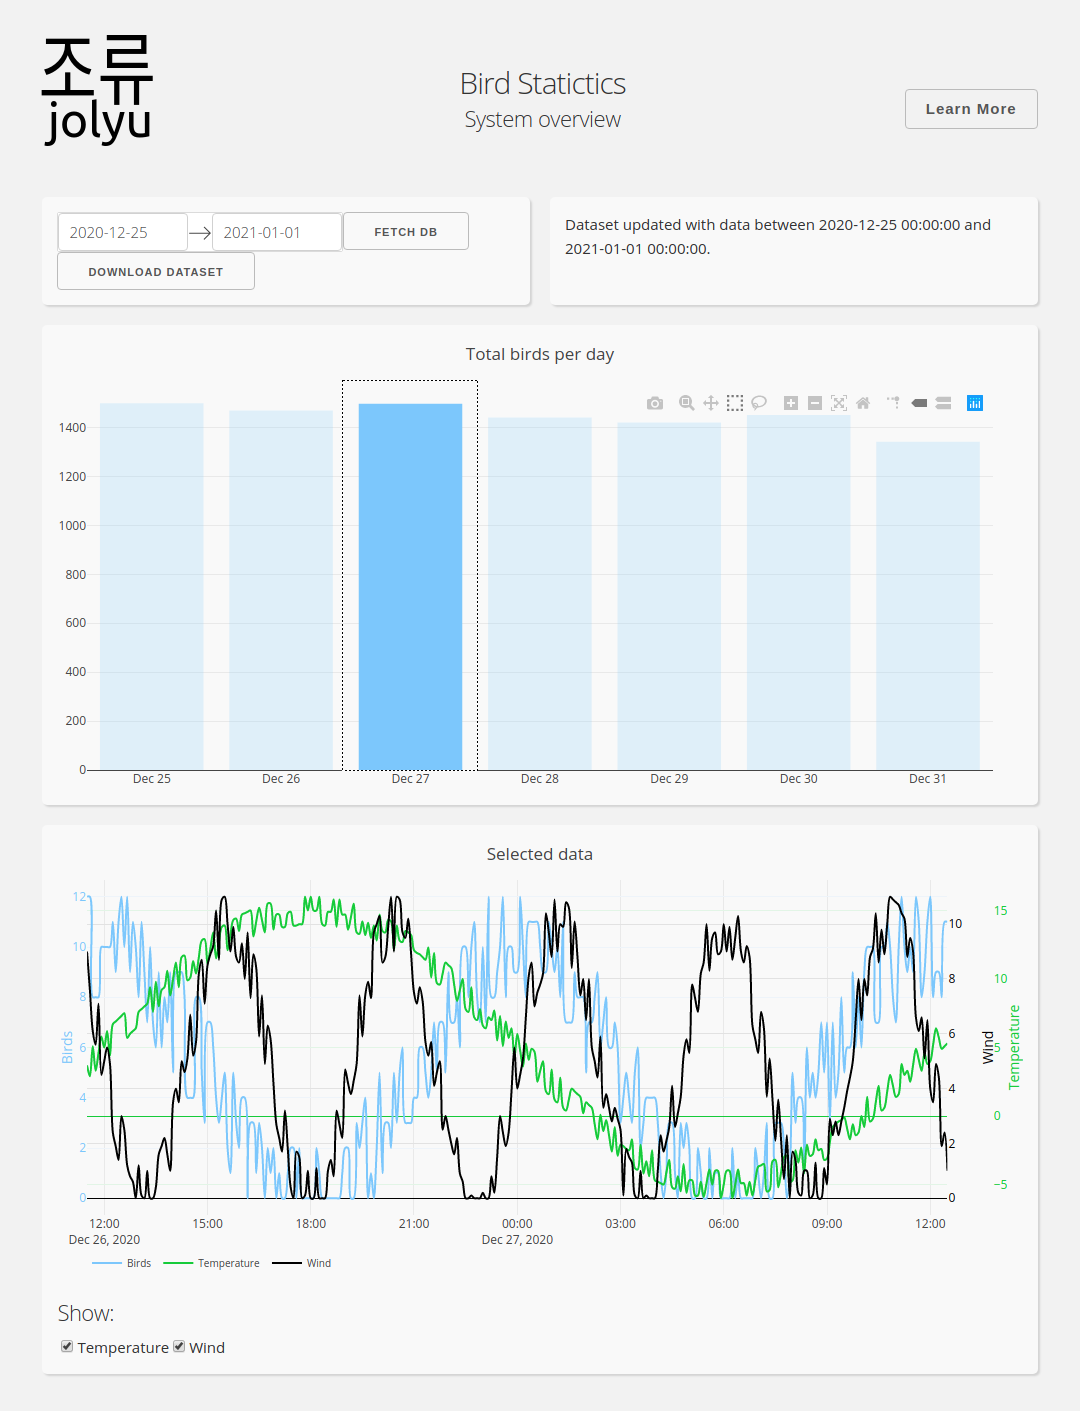
\includegraphics[width=.9\textwidth]{implementering/nettside/nettside.png}
    \caption{Eksempelnettside til jolyu.}
    \label{fig:nettside:nettside}
\end{figure}

Når nettsiden lastes inn, vil data fra databasen hentes fra nettet. 
Deretter prosesserer og filtrerer programmet dataen slik at det ikke bare er punktdata, men data basert på timer, dager, måneder og så videre. 
Dette krever effektive sortering- og filtreringsalgoritmer, da dataen kan inneholde flere tusen punkter.
Noen av disse algoritmene er allerede implementert i ferdige biblioteker, mens andre må implementeres med vanlige funksjoner i Python. 
Flyten på nettsiden kan sees i flytdiagrammet i \autoref{fig:nettside:flytdiagram}.

\begin{figure}[!htbp]
    \centering
    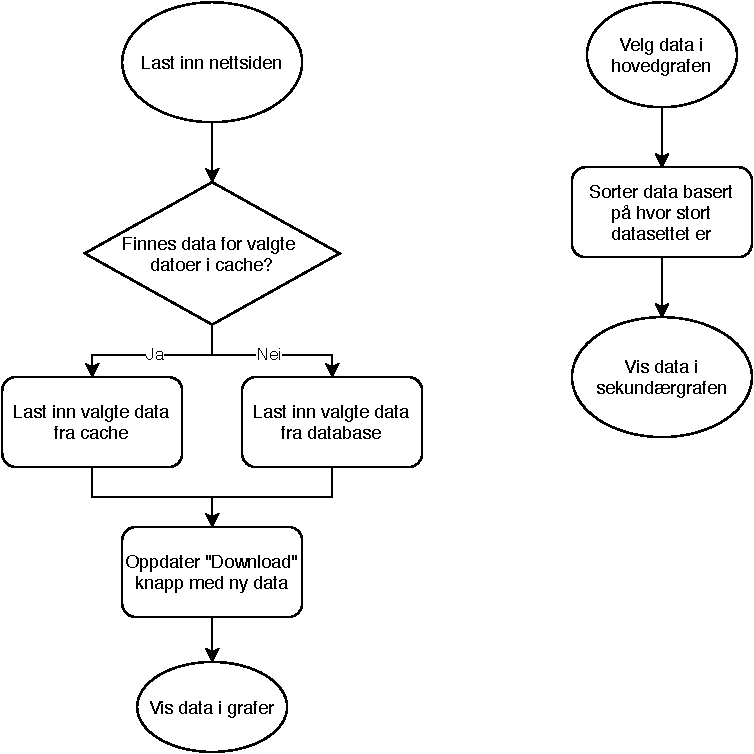
\includegraphics[width=.7\textwidth]{implementering/nettside/JolyuNettsideOverordnetFlyt.pdf}
    \caption{Flytdiagrammet til nettsiden.}
    \label{fig:nettside:flytdiagram}
\end{figure}

Store deler av nettsiden fungerer på samme måte. 
Det kjøres en funksjon om du velger noe data i en graf, eller ber nettsiden hente et nytt datasett. 
Dette registreres ved hjelp av en ''callback'', se \autoref{sec:impl:nettside:callback}.
Det vil derfor kun gis noen eksempler i avsnittene under, og koden til hele nettsiden kan leses på jolyu sin GitHub \cite{GitHub}, eller direkte til "repository": \url{https://github.com/jolyu/nettside}.

\subsubsection{Rammeverket}\label{sec:impl:nettside:rammeverk}

\textit{Dash} \cite{dash} er en kombinasjon og mellomledd mellom det pythonbaserte nettside-rammeverket for statiske nettsider, \textit{flask}, \cite{flask} og javascript biblioteket \textit{plotly} \cite{plotly} for å plotte data.

Dash fungerer ved å bruke spesialobjekter fra \textit{plotly} som ''graph'' og ''buttons'', og vanlige \html{html} objekter som \html{div} og \html{header}. 
Disse defineres i en liste med nøkkelverdier for variabler. Se \autoref{code:impl:nettside:dash1} som er tatt fra dokumentasjonen til \textit{Dash}. 

\begin{listing}[!htb]
\begin{minted}{python}
    import dash_core_components as dcc

    dcc.Dropdown(
        options=[
            {'label': 'New York City', 'value': 'NYC'},
            {'label': 'Montréal', 'value': 'MTL'},
            {'label': 'San Francisco', 'value': 'SF'}
        ],
        value='MTL'
    )
\end{minted}
\caption{Eksempel på hvordan implementere en enkel ''dropdown'' (valgliste) i dash.}
\label{code:impl:nettside:dash1}
\end{listing}

\textit{Flask} er i utgangspunktet laget for statiske nettsider, der data er ferdig laget når nettsiden lastes inn. 
Det Dash implementerer i \textit{flask}, er hvordan lage mer interaktive nettsider ved å legge til ''callbacks'', funksjoner som kjører når du for eksempel trykker på en knapp eller endrer på zoom i en graf.
Det er slik store deler av nettsiden er bygget opp, ved at brukeren endrer på hvilke objekter som er valgt eller drar i en slider. 
Da vil det skje en ''callback'' som vil kunne endre på data og deretter oppdatere nettsiden. 



\subsubsection{Callbacks}\label{sec:impl:nettside:callback}

Nettsiden bruker stort sett ''callbacks'' for å endre på hvilke data som skal vises i de forskjellige grafene. 
%Dersom det blir tatt utgangspunkt i en forenklet figur av nettsiden vist i \autoref{fig:impl:nettside:forenkletNettside} og \ref{fig:impl:nettside:callback}, kan vi s
En ''callback'' er en type funksjon som reagerer når noe endres på eller en hendelse, som et knappetrykk. 
Deretter kjøres funksjonen for så å returnere data til et annet objekt. 

\begin{figure}[!htbp]
    \centering
    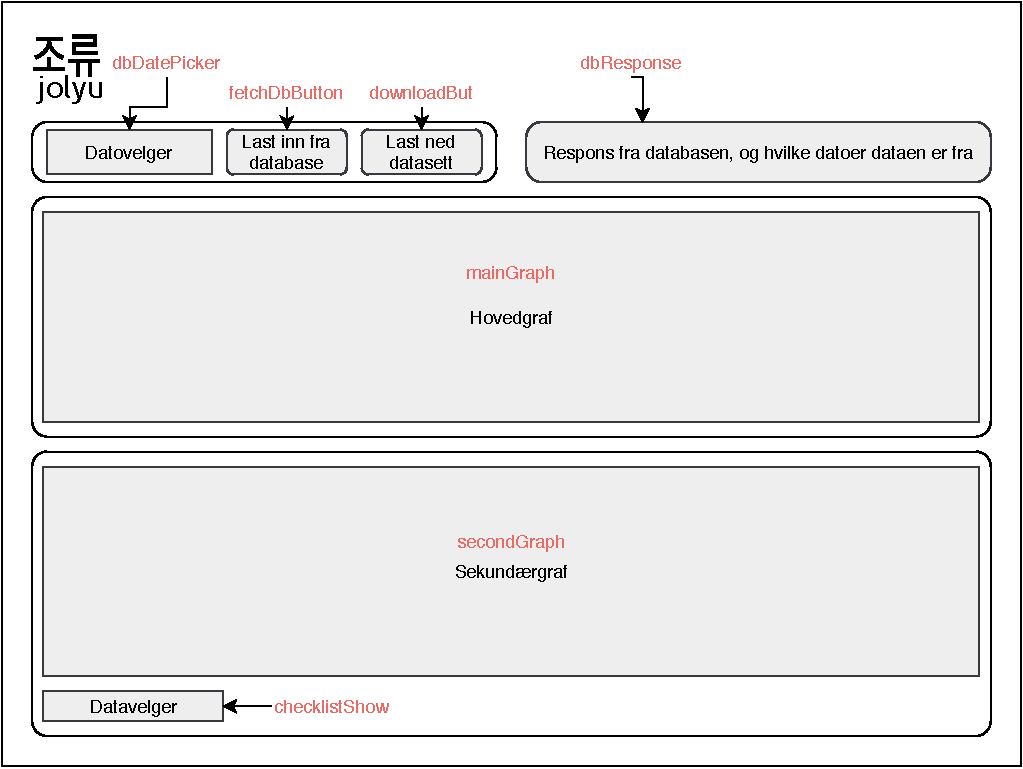
\includegraphics[width=0.9\textwidth]{implementering/nettside/NettsideEnkel.pdf}
    \caption{Forenklet figur av nettsiden med hva elementer i grå bokser og navnet til elementet i rød teks, eventuelt med pil til elementet.}
    \label{fig:impl:nettside:forenkletNettside}
\end{figure}

Alle de grå elementene i \autoref{fig:impl:nettside:forenkletNettside} brukes til å gjøre en ''callback'' for ulike ting. 
De røde navnene er navnene på elementene som vil kjøre en ''callback''.
Figur \ref{fig:impl:nettside:callback} viser hvordan ''callbacks'' flytter data rundt om på siden. 
Ta \python{fetchDbButton} som eksempel. 
Når knappen klikkes på, vil data skrives til alle stedene pilene peker til. 
Der de blå boksene med tekst er forskjellige atributter i hvert av elementene.


\begin{figure}[!htbp]
    \centering
    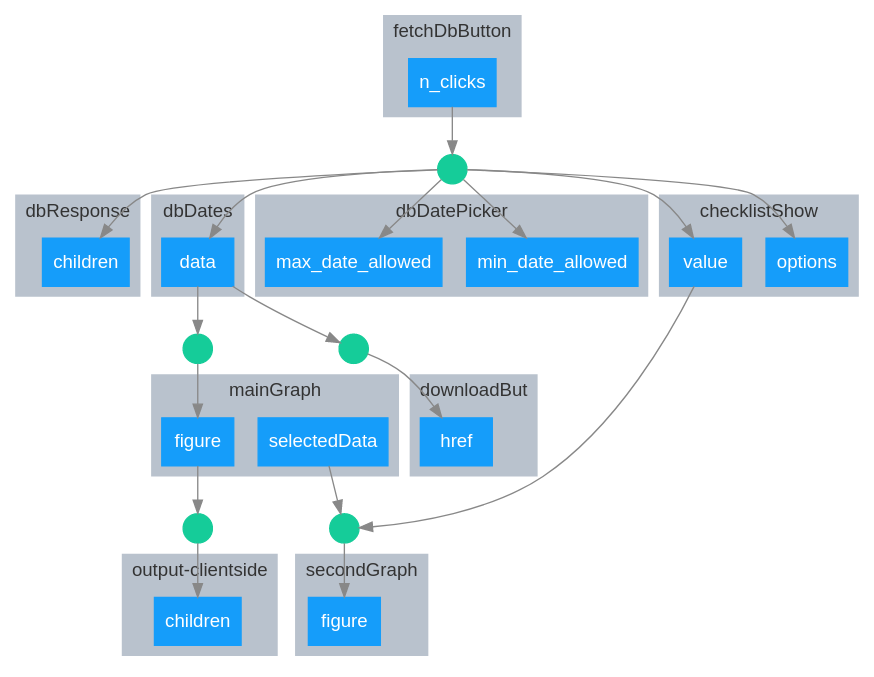
\includegraphics[width=.9\textwidth]{implementering/nettside/callbacks.png}
    \caption{''Callback''-diagram for nettsiden. De grønne nodene er et callback som utløses av det som kommer inn, og skriver til der pilene peker.}
    \label{fig:impl:nettside:callback}
\end{figure}

Når \python{dbDates} oppdateres, trigger det to forskjellige ''callbacks''. 
Den ene vil oppdatere \html{href} i \python{downloadBut} med nedlastning av det aktive datasettet, og den andre vil oppdatere hovedgrafen.
I \autoref{code:impl:nettside:callback} vises det hvordan ''callback''-en for oppdatering av nedlastning fungerer. 

\begin{listing}[!htb]
\begin{minted}{python}
    @app.callback(
        Output("downloadBut", "href"),
        [
            Input("dbDates", "data"),
        ]
    )
    def UpdateDownloadButton(dates):
        """ Updates the download button with the data from the current dataset """
        # Check if the dates variable is not empty
        if dates == None:
            dates = GetInitialDates(ref, initialDays)
        else:
            dates = pd.to_datetime(dates)
        
        # Query the dataset
        df = QueryDF(ref, dates)
    
        # Convert dataframe to csv and convert into a "file" that is parsed into a 
        # string with no invalid characters
        csvString = df.to_csv(encoding="utf-8")
        csvString = "data:text/csv;charset=utf-8," + urlParse.quote(csvString)
        return csvString
\end{minted}
\caption{''Callback'' som oppdaterer nedlastningen av det aktive datasettet, basert på en oppdatering av aktive datoer i datasettet.}
\label{code:impl:nettside:callback}
\end{listing}

En ''callback'' initialiseres ved å si hva som skal være \python{Input} (en type ''trigger'') og hvor data skal plasseres når ''callback'' er ferdig med en \python{Output}. 
I dette tilfellet vil ''callback''-en kjøres når \python{dbDates} endres. 
Denne inneholder første og siste dato i det aktive datasettet. 
Denne oppdateres av \python{fetchDbButton}, som henter datasettet fra databasen, som vist i \autoref{fig:impl:nettside:callback}. 
Den vil deretter lage en \python{string} med alle aktive datasett og plassere det som en link i atributten \html{href}.

Dette er bare en av ''callback''-ene på nettsiden, for å se hele nettsiden kan en gå til jolyu sin GitHub \cite{GitHub}.

\subsubsection{Sortering og filtrering}\label{sec:impl:nettside:sortering}

Sortering og filtrering kan gjøres på mange måter. 
Det enkleste og ofte det beste er å bruke innebygde funksjoner. 
På nettsiden brukes en avansert liste, en \python{dataframe} fra \textit{pandas} \cite{dataframe}. 
Den har sine egne sorteringsalgoritmer som brukes aktivt på nettsiden. 

Den mest intense sorteringen er å samle all punktdataen til måneder (eller uker/dager). 
Da det kan være flere hundretusen datapunkter, og sorteringsalgoritmen må derfor være effektiv. 
Derfor brukes de innebygde funksjonene for akkurat dette formålet. 
I \autoref{code:impl:nettside:sortering1} kan det ses hvordan funksjonen \python{dataframe.resample(<timegroup>).sum()} brukes for å summere alle punkter i en måned, sammen til et enkelt punkt.

\begin{listing}[!htb]
\begin{minted}{python}
    def DataToMonths(df):
        """ Sort data in dataframe into months """
        df = df.resample('M').sum()
        return df
    
    
    def DataToWeeks(df):
        """ Sort data in dataframe into weeks """
        df = df.resample('W').sum()
        return df
\end{minted}
\caption{Funksjoner som sorterer punkter på måneder og uker.}
\label{code:impl:nettside:sortering1}
\end{listing}

For å hente ut en liten del av datasettet brukes noen selvlagde funksjoner. 
I \python{FilterData(df, startDate, endDate)} sendes en dataframe, startdato og sluttdato inn. 
Funksjonen vil finne de aktuelle datapunktene som er innenfor dette tidsintervallet og returnere en ny dataframe.

\begin{listing}[!htb]
\begin{minted}{python}
    def FilterData(df, startDate, endDate):
        """ Filter out a partition of a dataframe """
        dff = df.loc[(df.index > startDate)
            & (df.index < endDate)]
        return dff
\end{minted}
\caption{Funksjon som henter ut et område innenfor to gitte datoer.}
\label{code:impl:nettside:sortering2}
\end{listing}


\subsubsection{Database}\label{sec:impl:nettside:database}

Kommunikasjon mellom Pi-en og nettsiden går via Google sin ''Realtime Firebase'' database. 
Denne kommunikasjonen foregår over Wi-Fi. 
Dataene Pi-en samler inn blir sendt til databasen som \textit{dictionaries} og lagret der på et NoSQL-format. 
En NoSQL-database er ikke like streng med struktur i forhold til en SQL-database, så den takler bedre endringer i strukturen til dataene. 
Firebase har Python-bibliotek for overføring mellom prosesseringsenhet og databasen, og fra databasen til nettsiden. 
Måten dette fungerer på blir abstrahert bort av ferdigutviklet software, som ligger i \textit{firebase\_admin} biblioteket. 
All data i databasen har en nøkkel som er et tidsstempel\footnote{Unix tidsstempel (eng: Unix Timestamp) - Tid i sekunder fra 1. januar 1970. Brukes mye i datateknologi.} som angir når det ble lastet opp i databasen. 
Når data blir hentet fra databasen kan det sorteres etter nøklene eller de forskjellige dataene som ligger innenfor hovednøkkelen.
Et eksempel på en slik database er en enkel \html{json}\footnote{Dette er en skriftlig versjon av en dictionary. Noe som kan lagres i en fil.}-liste, som sett i \autoref{code:impl:nettside:json}.

\begin{listing}[!htb]
    \begin{minted}{json}
    {
        "1609455600": {
            "time": 1609455600.0, 
            "birds": 8.0, 
            "Temperature": 7.5, 
            "Wind": 0.1, 
            "Pressure": 1027.8,
        }  
    }
    \end{minted}
    \caption{Enkel data i json. Som også er slik data er lagret i databasen. Dette er også en bra måte å visualisere en \textit{dictionary}.}
    \label{code:impl:nettside:json}
\end{listing}

\newpage
\subsection{Strukturelt}\label{sec:impl:struktur}

Metallstativet som boksen og værstasjonen skal festes til, er vist i \autoref{fig:Stativ}. 
Her vil boksen festes til stangen $\SI{1}{\meter}$ over bakken med modulene til værstasjonen festet øverst, $\SI{1.5}{\meter}$ over bakken. 
%Stativet vil plasseres på flatt underlag som spesifisert i systemkrav \idref{id:underlag}. 
Kamera festes inne i boksen bak den skrå delen for at regn, snø og andre fremmedlegemer ikke skal samle seg foran linsen, og for at det skal være vinklet mot himmelen. 
Boksen printes i PLA-plast på en 3D-printer, og er designet for å kunne stå utendørs over lengre tid.

\todo{Burde skrive noe om hvordan vi skal forhindre at den faller. Feks vaier/tråd ned i bakken som en pyramide}

\begin{figure}[!htbp]
    \centering
    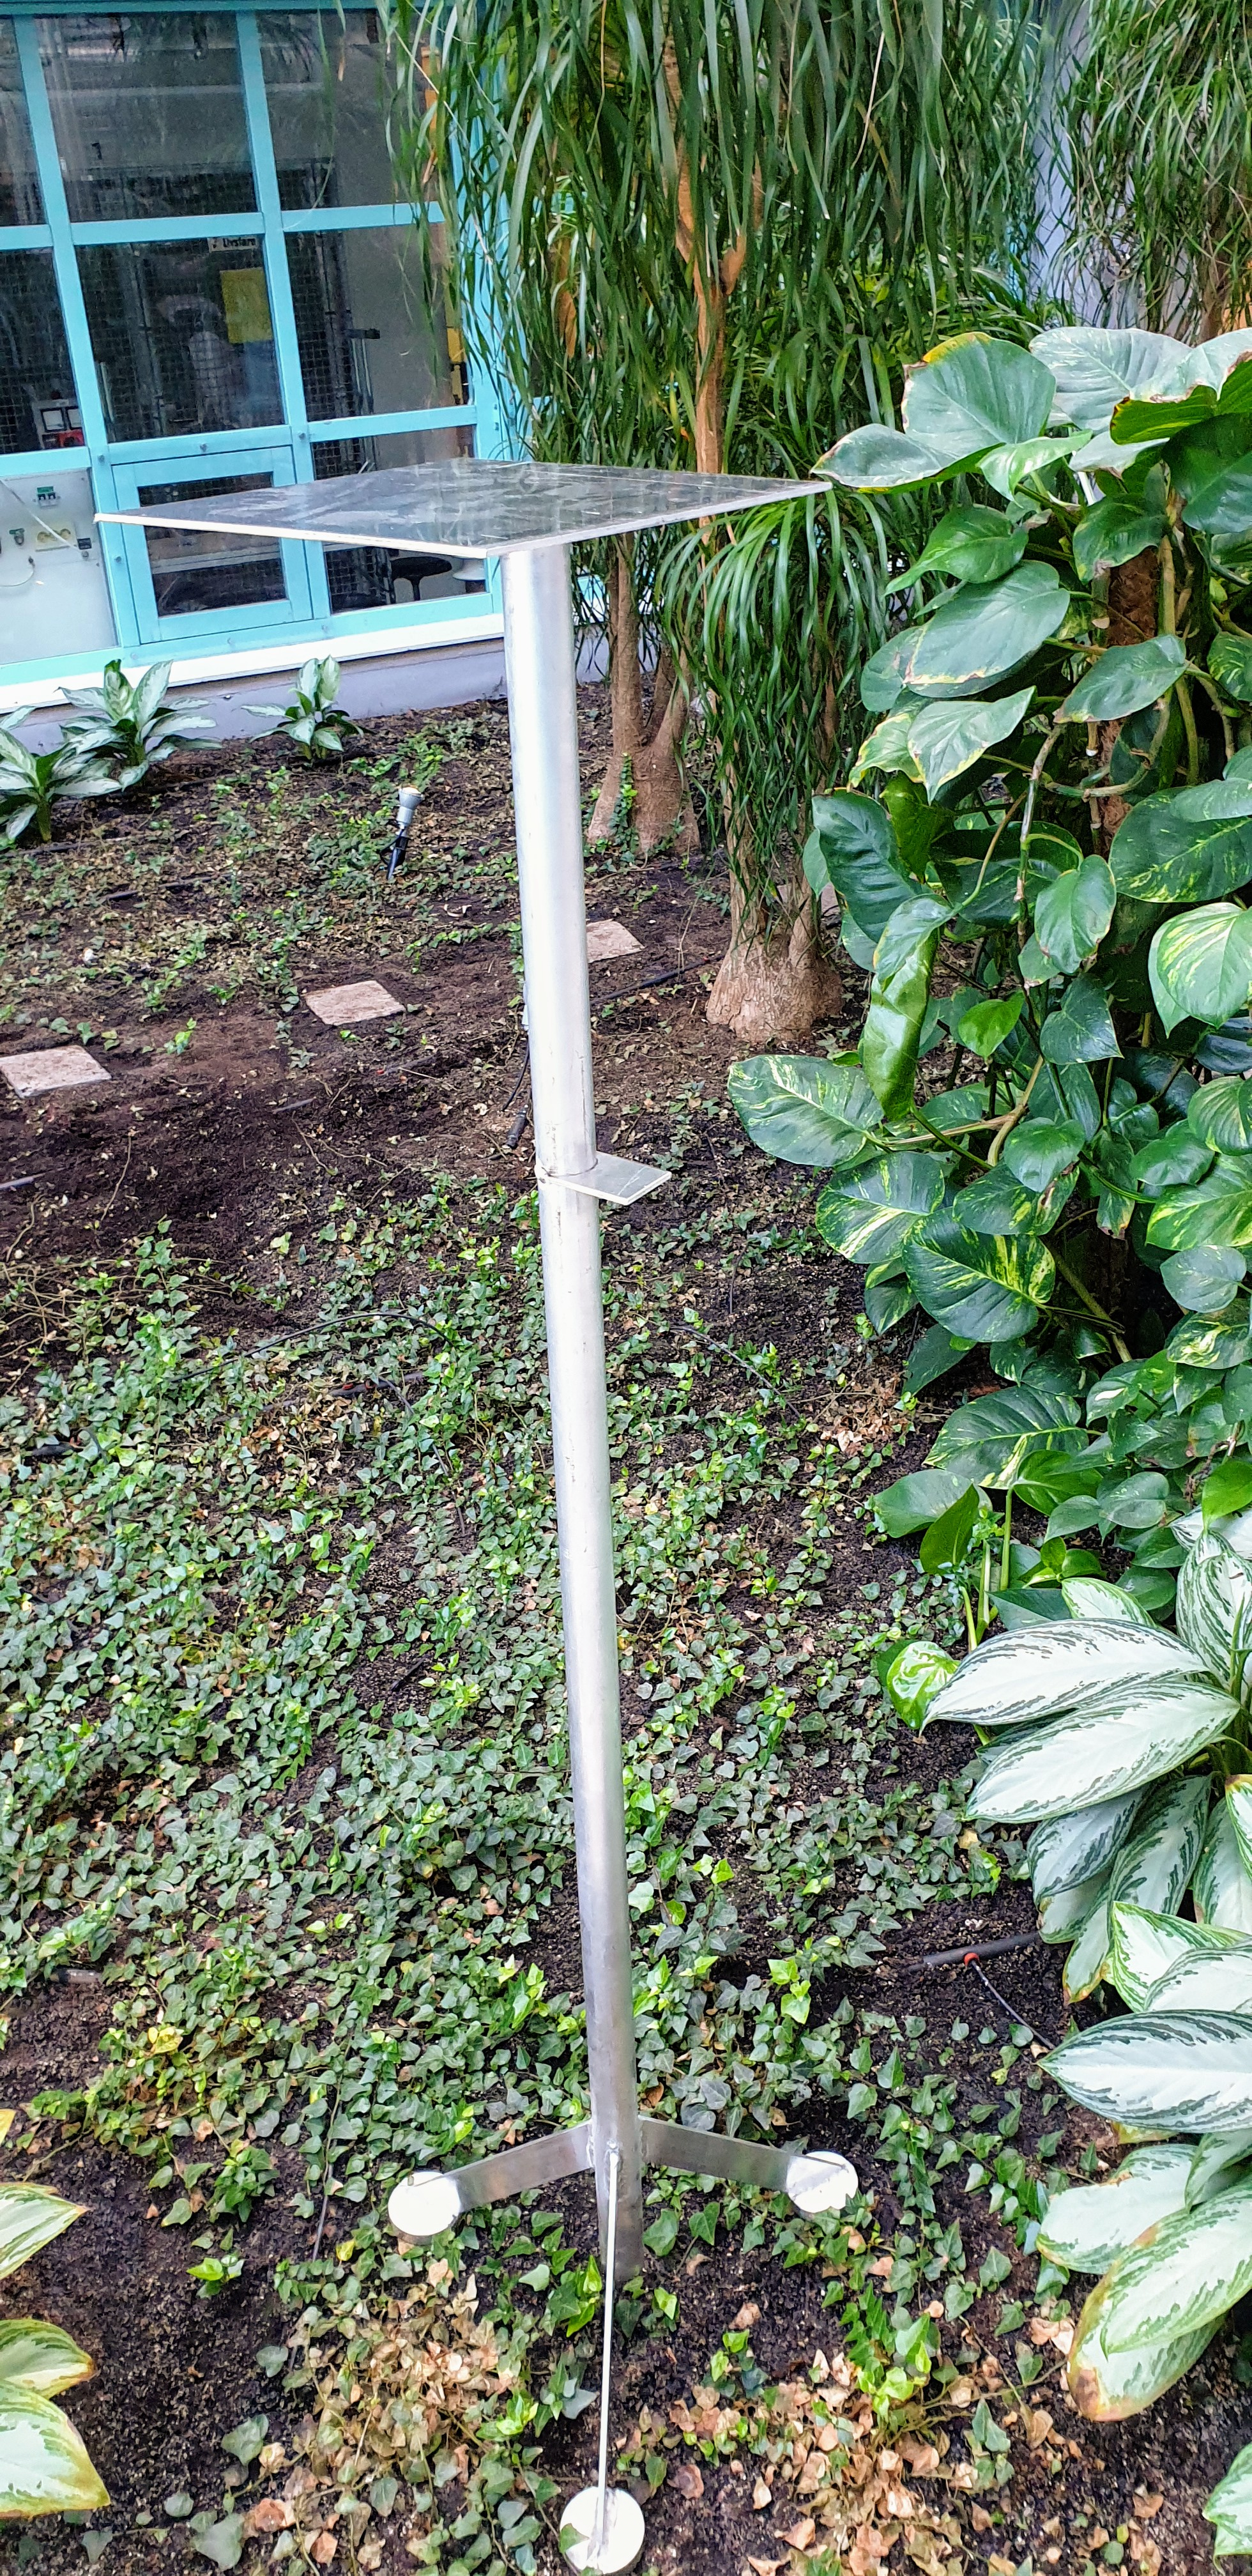
\includegraphics[trim={0 0 0 20cm}, clip, width=.5\textwidth]{implementering/Stativ.jpg}
    \caption{Stativ for boks og værstasjon.}
    \label{fig:Stativ}
\end{figure}

En 3D-modell av boksen er vist i figur \ref{fig:boks}, og en 3D-modell av strukturen til hele systemet er vist i figur \ref{fig:3dsystem}.

\begin{figure}[!htbp]
\centering
\begin{minipage}[c]{0.45\textwidth}
\centering
    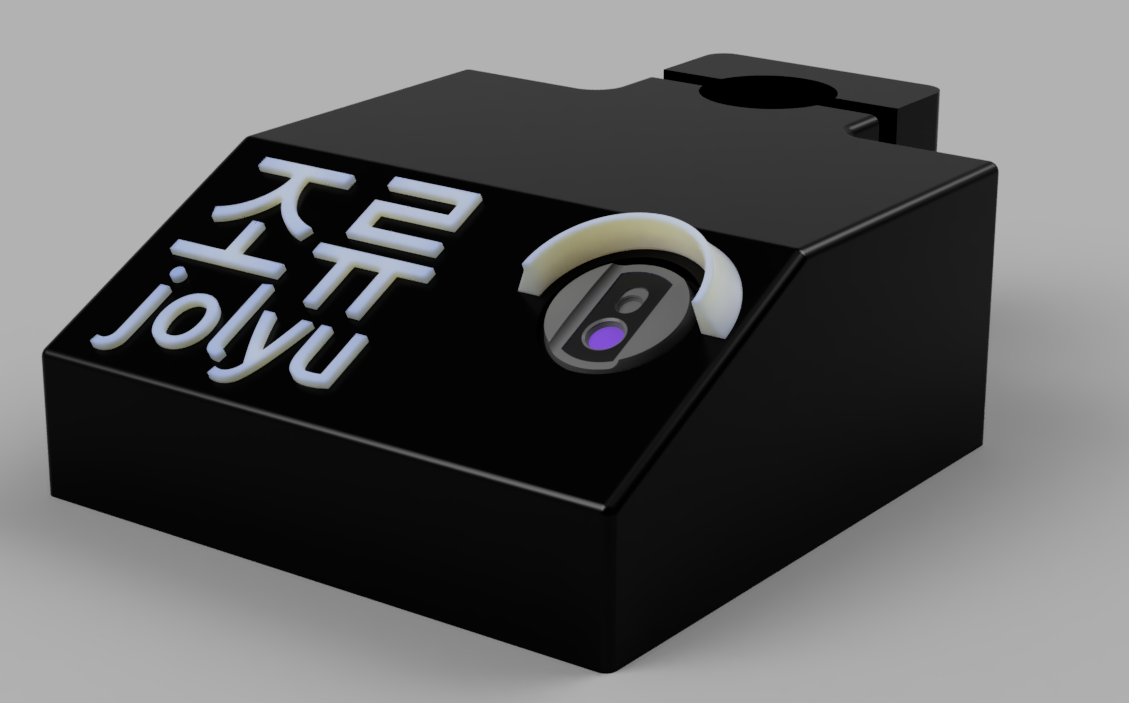
\includegraphics[width=0.9\textwidth]{implementering/Boks_render.png}
    \caption{En 3D-modell av boksen som skal holde kamera og prosesseringsenhet.}
    \label{fig:boks}
    
\end{minipage}
\begin{minipage}[c]{0.45\textwidth}
\centering
    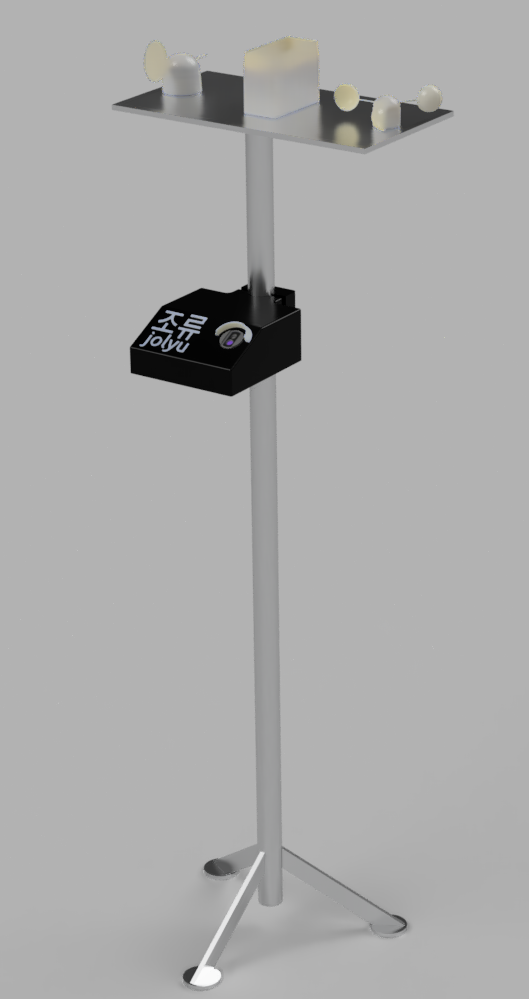
\includegraphics[width=0.9\textwidth]{implementering/stativ_render.png}
    \caption{En 3D-modell av hele systemets fysiske realisering.}
    \label{fig:3dsystem}
\end{minipage}
\end{figure}

\section{Verifikasjon og test}
\label{sec:verifikasjon}
\textit{Her dokumenteres hvordan systemet er testet. Resultat av test og drøfting av potensielle forbedringer. Det er viktig å få med at systemet eller deler av systemet virker eller ikke virker. Dersom det er mulig å tallfeste \textbf{hvor godt} systemet virker, er det bra.}



% SKal endre til bibtex %

%Bibliografi: Legg til flere elementer ved å legge til flere \bibitem:--------
\phantomsection
\addcontentsline{toc}{section}{Referanser}
\begin{thebibliography}{99}

\bibitem{bibelen}
  Albert Einstein,
  \emph{Elektronikkbibelen},
  O Store Forlag,
  1. utgave,
  1930.

\end{thebibliography}


% Vedlegg
% Legge til flere vedlegg-filer i mappen og legge til flere input
\appendix
%Tillegg. Flere tillegg legges til ved å lage flere sections:-----------------
\section{Vedlegg 1}
\label{sec:vedlegg1}
\textit{Ikke-nummerert rapportdel der det kan legges stoff som kan være av aktuelt for spesielt interesserte lesere og som ville redusert lesbarheten om det hadde vært inkludert i hovedteksten. Eksempler kan være større tabeller eller fullstendig kildekode.}

\textbf{Må teste noe greier}


\end{document}